% One figure per training width, one thin curve per seed (no averaging),
% generated by plot_modelbased_seed_curves.py --run exp2_try3_210x300 --method lista --metric rf.
% Requires \usepackage{graphicx} and \usepackage{subcaption}. Paths are
% relative to the repo root (Figs/...); adjust \graphicspath or the paths below.
% Include with: % One figure per training width, one thin curve per seed (no averaging),
% generated by plot_modelbased_seed_curves.py --run exp2_try3_210x300 --method lista --metric rf.
% Requires \usepackage{graphicx} and \usepackage{subcaption}. Paths are
% relative to the repo root (Figs/...); adjust \graphicspath or the paths below.
% Include with: % One figure per training width, one thin curve per seed (no averaging),
% generated by plot_modelbased_seed_curves.py --run exp2_try3_210x300 --method lista --metric rf.
% Requires \usepackage{graphicx} and \usepackage{subcaption}. Paths are
% relative to the repo root (Figs/...); adjust \graphicspath or the paths below.
% Include with: % One figure per training width, one thin curve per seed (no averaging),
% generated by plot_modelbased_seed_curves.py --run exp2_try3_210x300 --method lista --metric rf.
% Requires \usepackage{graphicx} and \usepackage{subcaption}. Paths are
% relative to the repo root (Figs/...); adjust \graphicspath or the paths below.
% Include with: \input{Figs/multifigure/lista_seed_curves_exp2_try3_210x300_figure}
\begin{figure}[htbp]
\centering
\begin{subfigure}[t]{\linewidth}
  \centering
  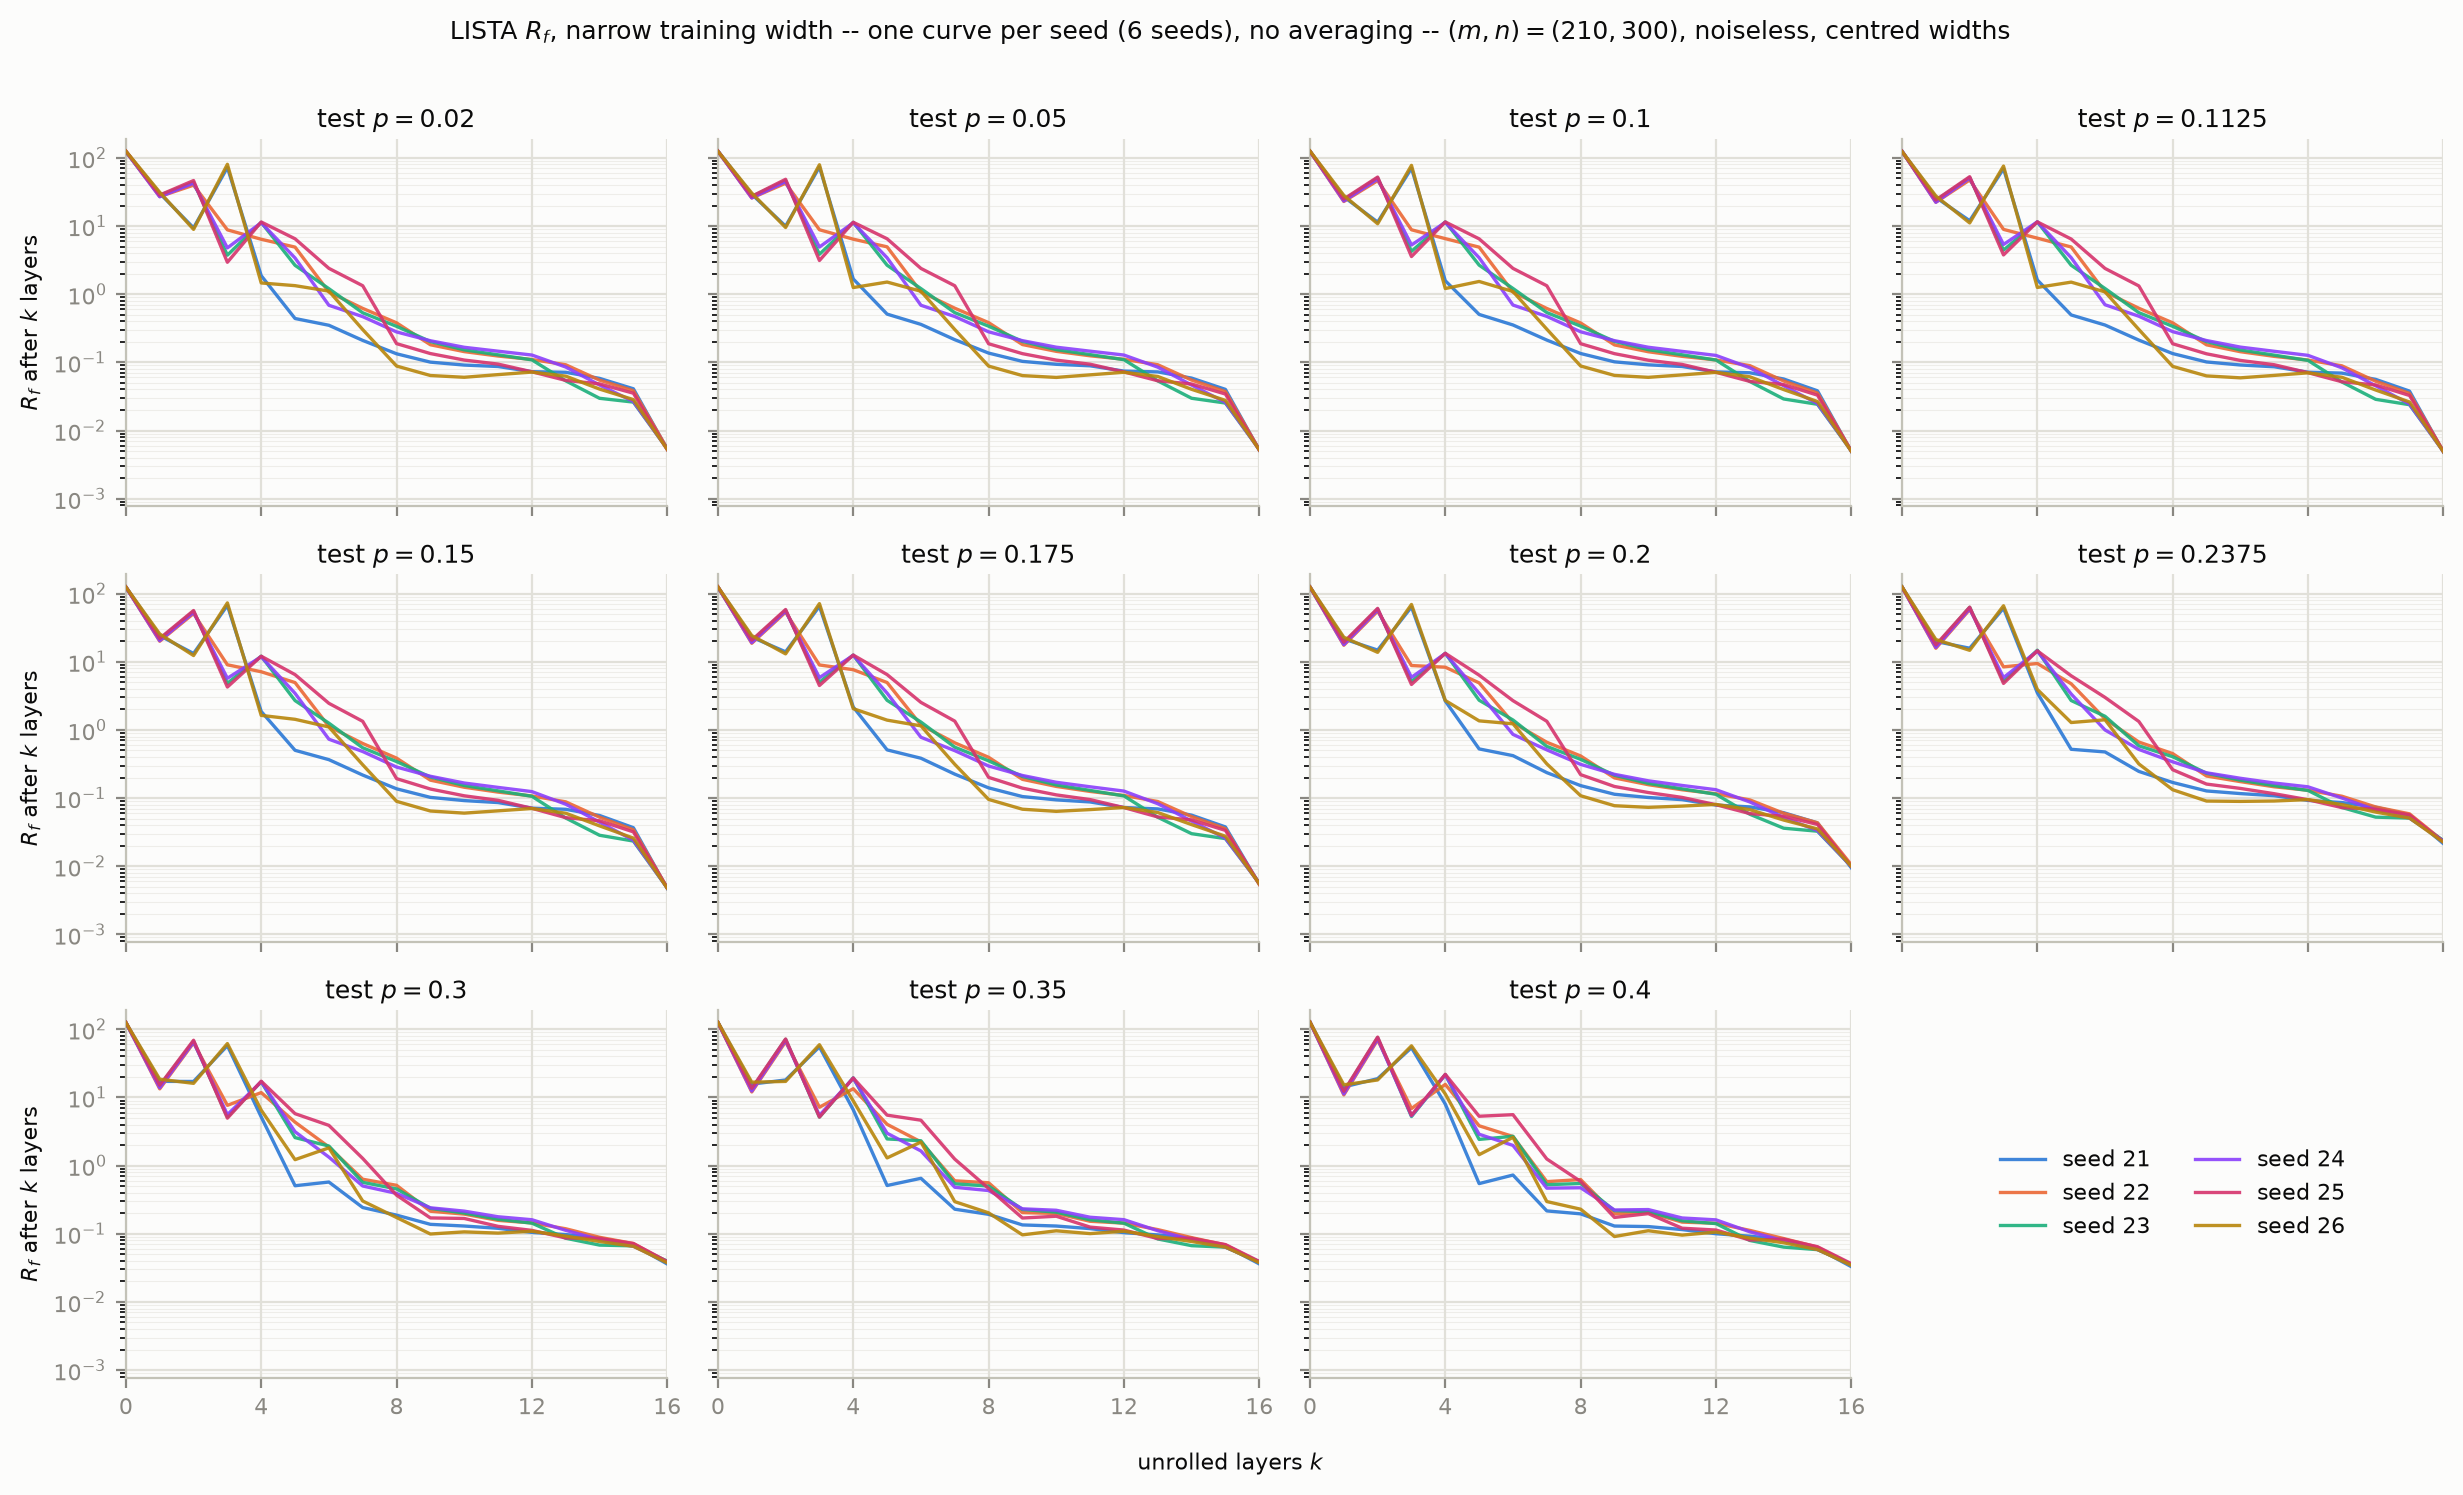
\includegraphics[width=\linewidth]{Figs/exp2_try3_210x300/lista_seed_curves_exp2_try3_210x300_narrow.png}
  \caption{Narrow ($p = 0.175$)}
  \label{fig:lista-seed-curves-exp2-try3-210x300-narrow}
\end{subfigure}\\[6pt]
\begin{subfigure}[t]{\linewidth}
  \centering
  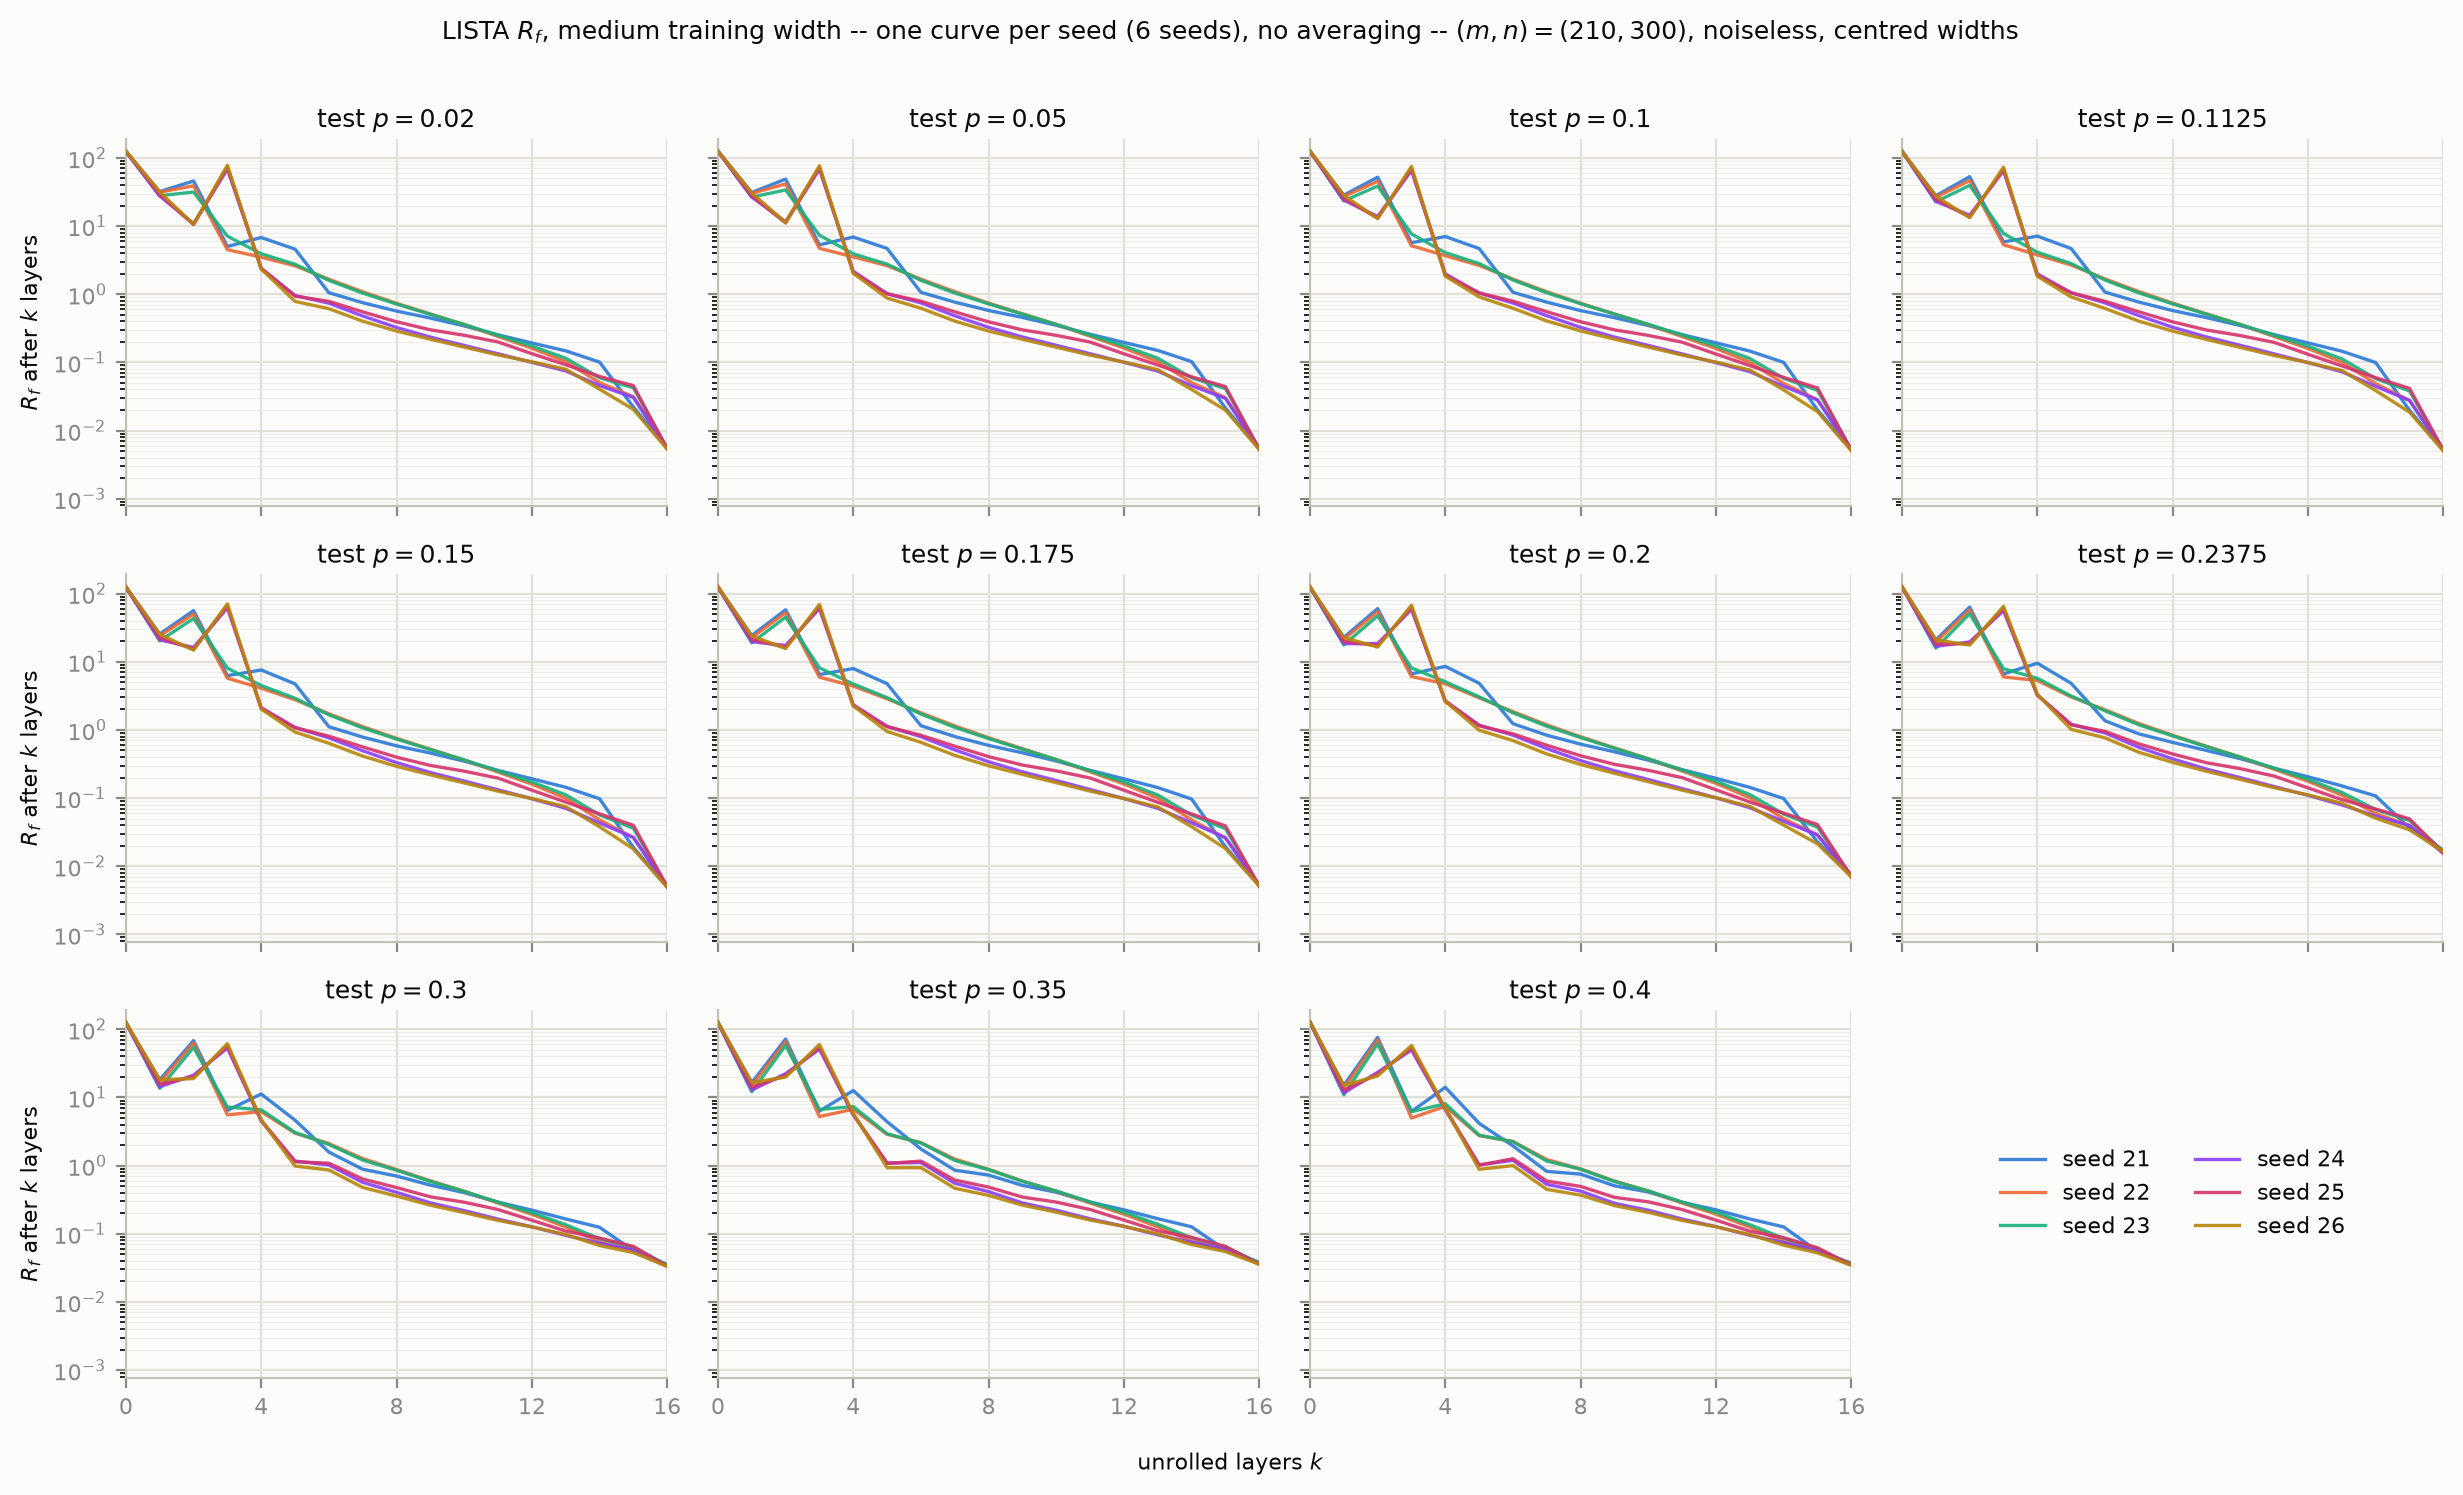
\includegraphics[width=\linewidth]{Figs/exp2_try3_210x300/lista_seed_curves_exp2_try3_210x300_medium.png}
  \caption{Medium ($p \in [0.1125, 0.2375]$)}
  \label{fig:lista-seed-curves-exp2-try3-210x300-medium}
\end{subfigure}\\[6pt]
\begin{subfigure}[t]{\linewidth}
  \centering
  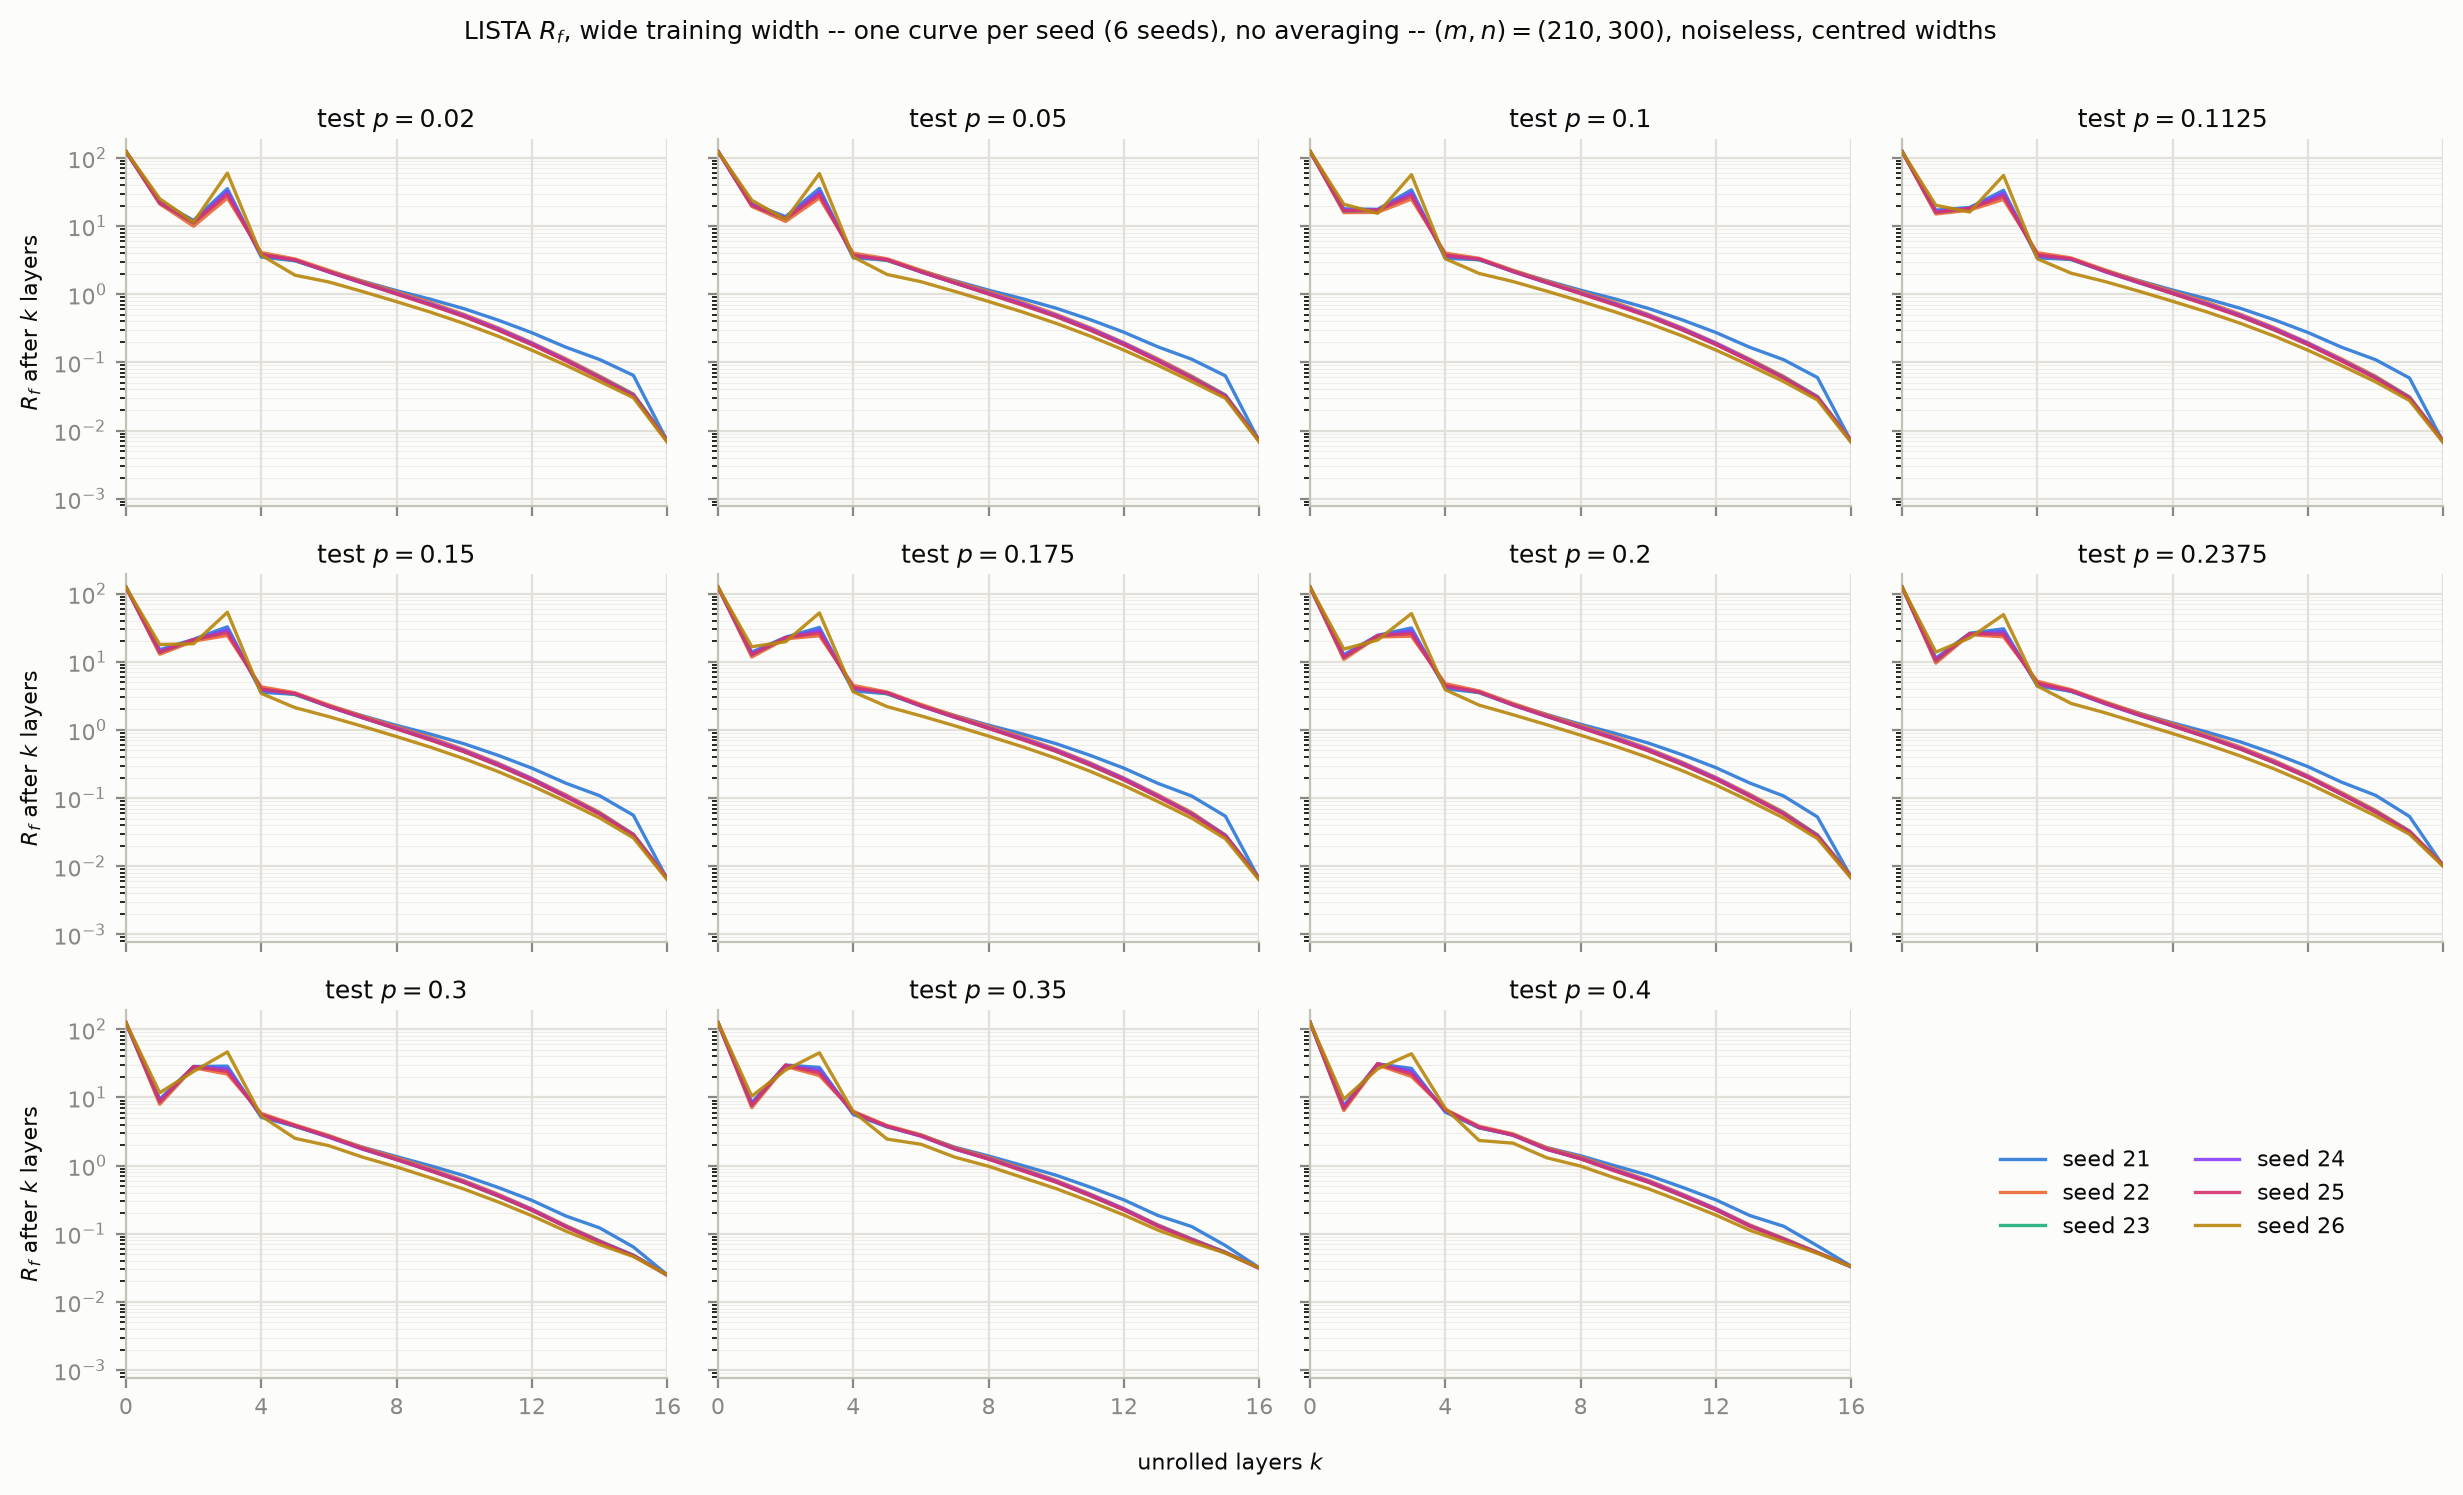
\includegraphics[width=\linewidth]{Figs/exp2_try3_210x300/lista_seed_curves_exp2_try3_210x300_wide.png}
  \caption{Wide ($p \in [0.05, 0.30]$)}
  \label{fig:lista-seed-curves-exp2-try3-210x300-wide}
\end{subfigure}\\[6pt]
\caption{LISTA, modified relative loss $R_f$ (Eq.~10) against unrolled layer $k$, $(m,n) = (210, 300)$, noiseless, centred widths. One curve per training seed (6 independently trained networks per width), no averaging; one panel per test sparsity $p$. $k = 0$ is the shared seeded start $x_0$, $k = 16$ the network's output. Unlike the model-free optimizer, every layer's weights are free, so the seeds may separate from the first layer on.}
\label{fig:lista-seed-curves-exp2-try3-210x300}
\end{figure}

\begin{figure}[htbp]
\centering
\begin{subfigure}[t]{\linewidth}
  \centering
  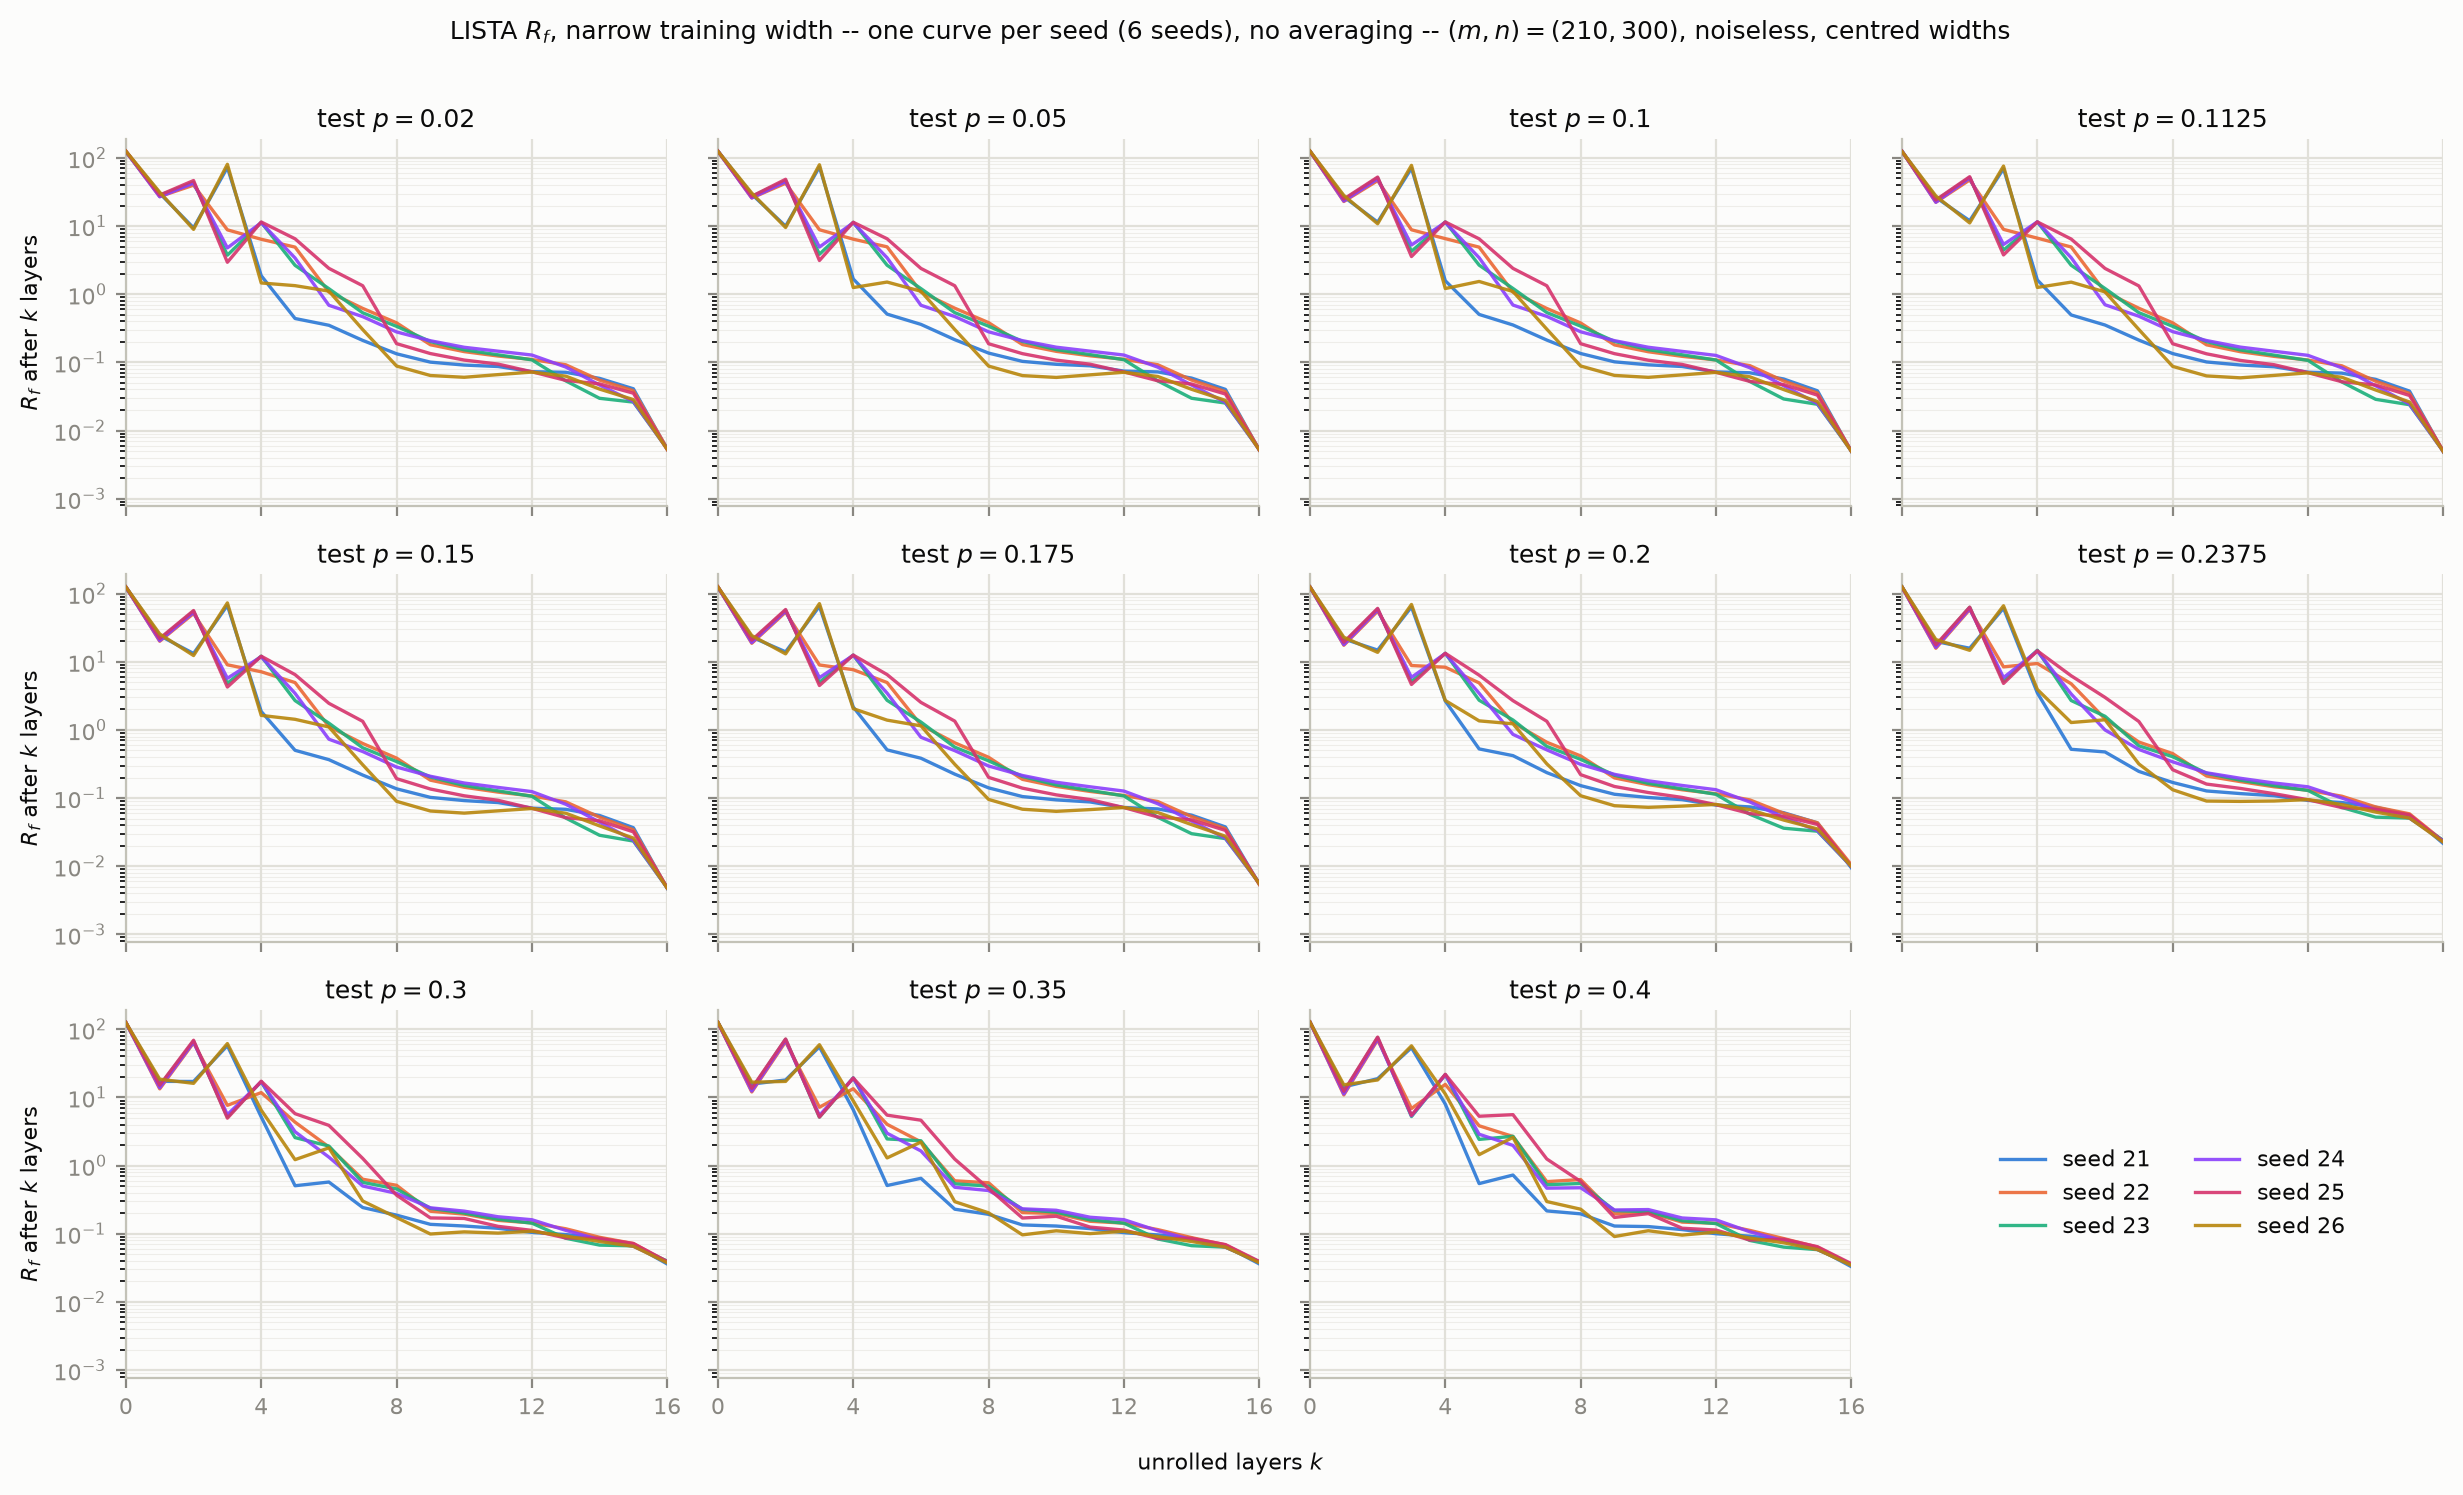
\includegraphics[width=\linewidth]{Figs/exp2_try3_210x300/lista_seed_curves_exp2_try3_210x300_narrow.png}
  \caption{Narrow ($p = 0.175$)}
  \label{fig:lista-seed-curves-exp2-try3-210x300-narrow}
\end{subfigure}\\[6pt]
\begin{subfigure}[t]{\linewidth}
  \centering
  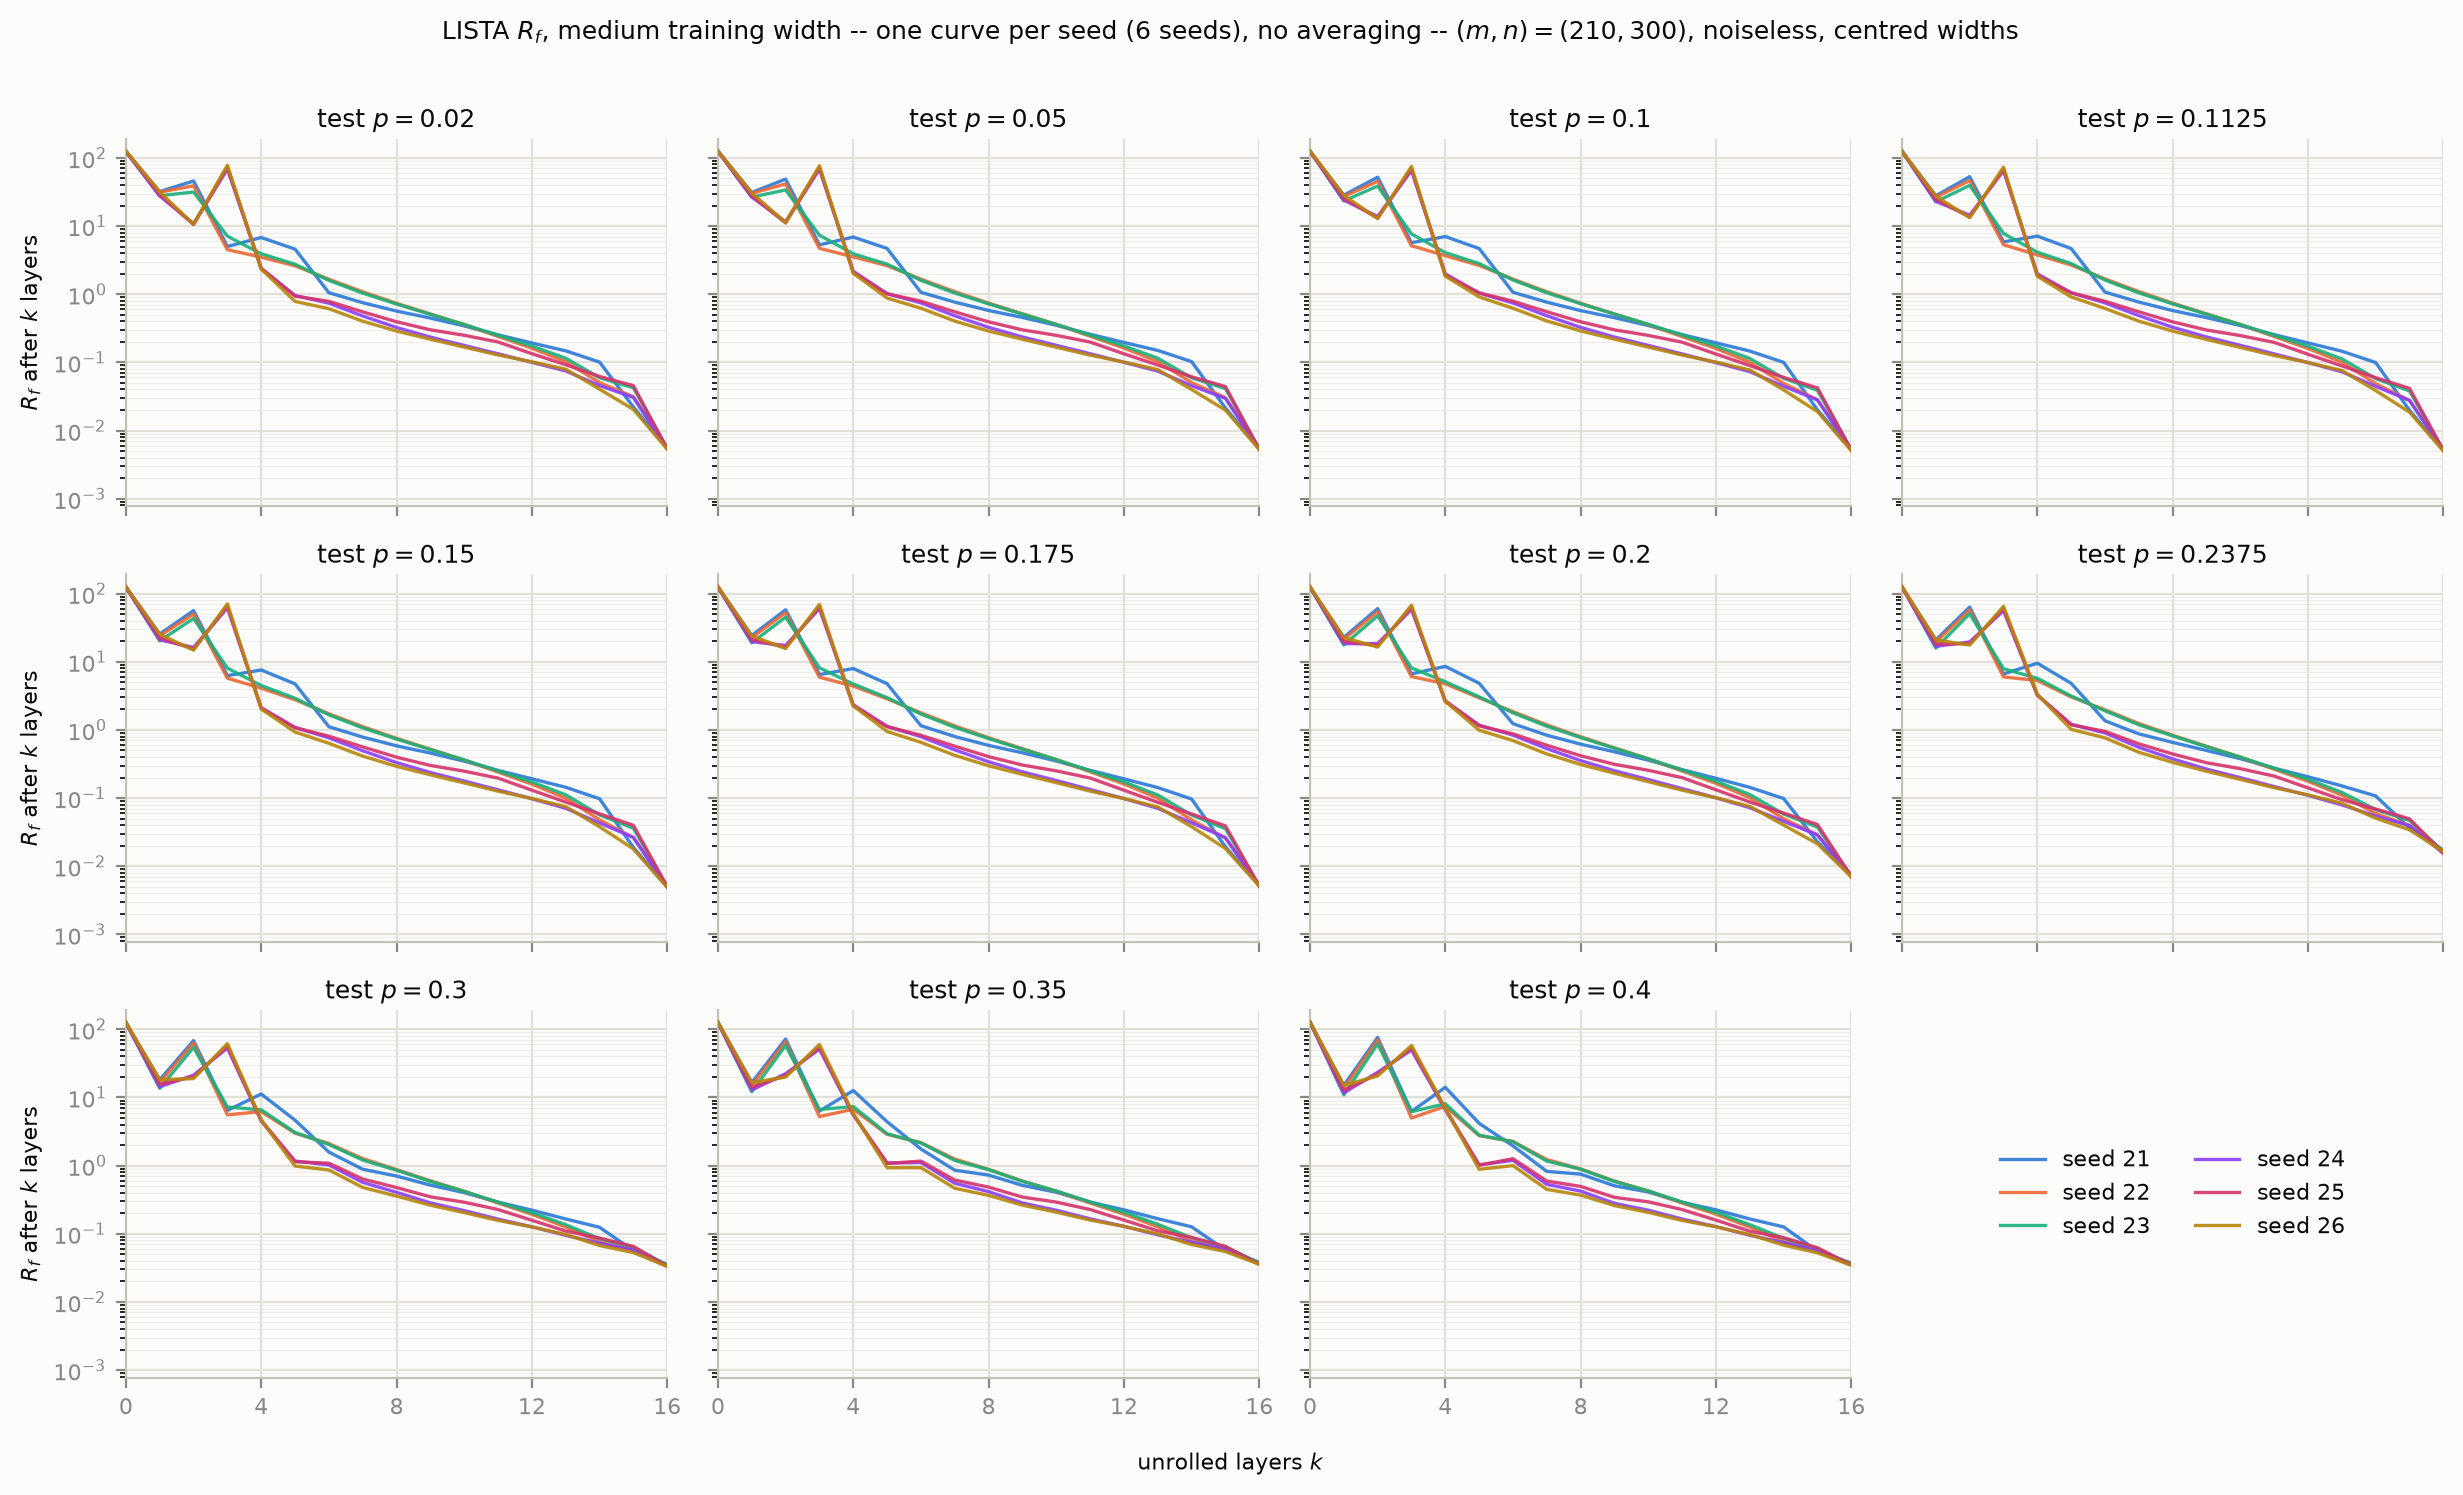
\includegraphics[width=\linewidth]{Figs/exp2_try3_210x300/lista_seed_curves_exp2_try3_210x300_medium.png}
  \caption{Medium ($p \in [0.1125, 0.2375]$)}
  \label{fig:lista-seed-curves-exp2-try3-210x300-medium}
\end{subfigure}\\[6pt]
\begin{subfigure}[t]{\linewidth}
  \centering
  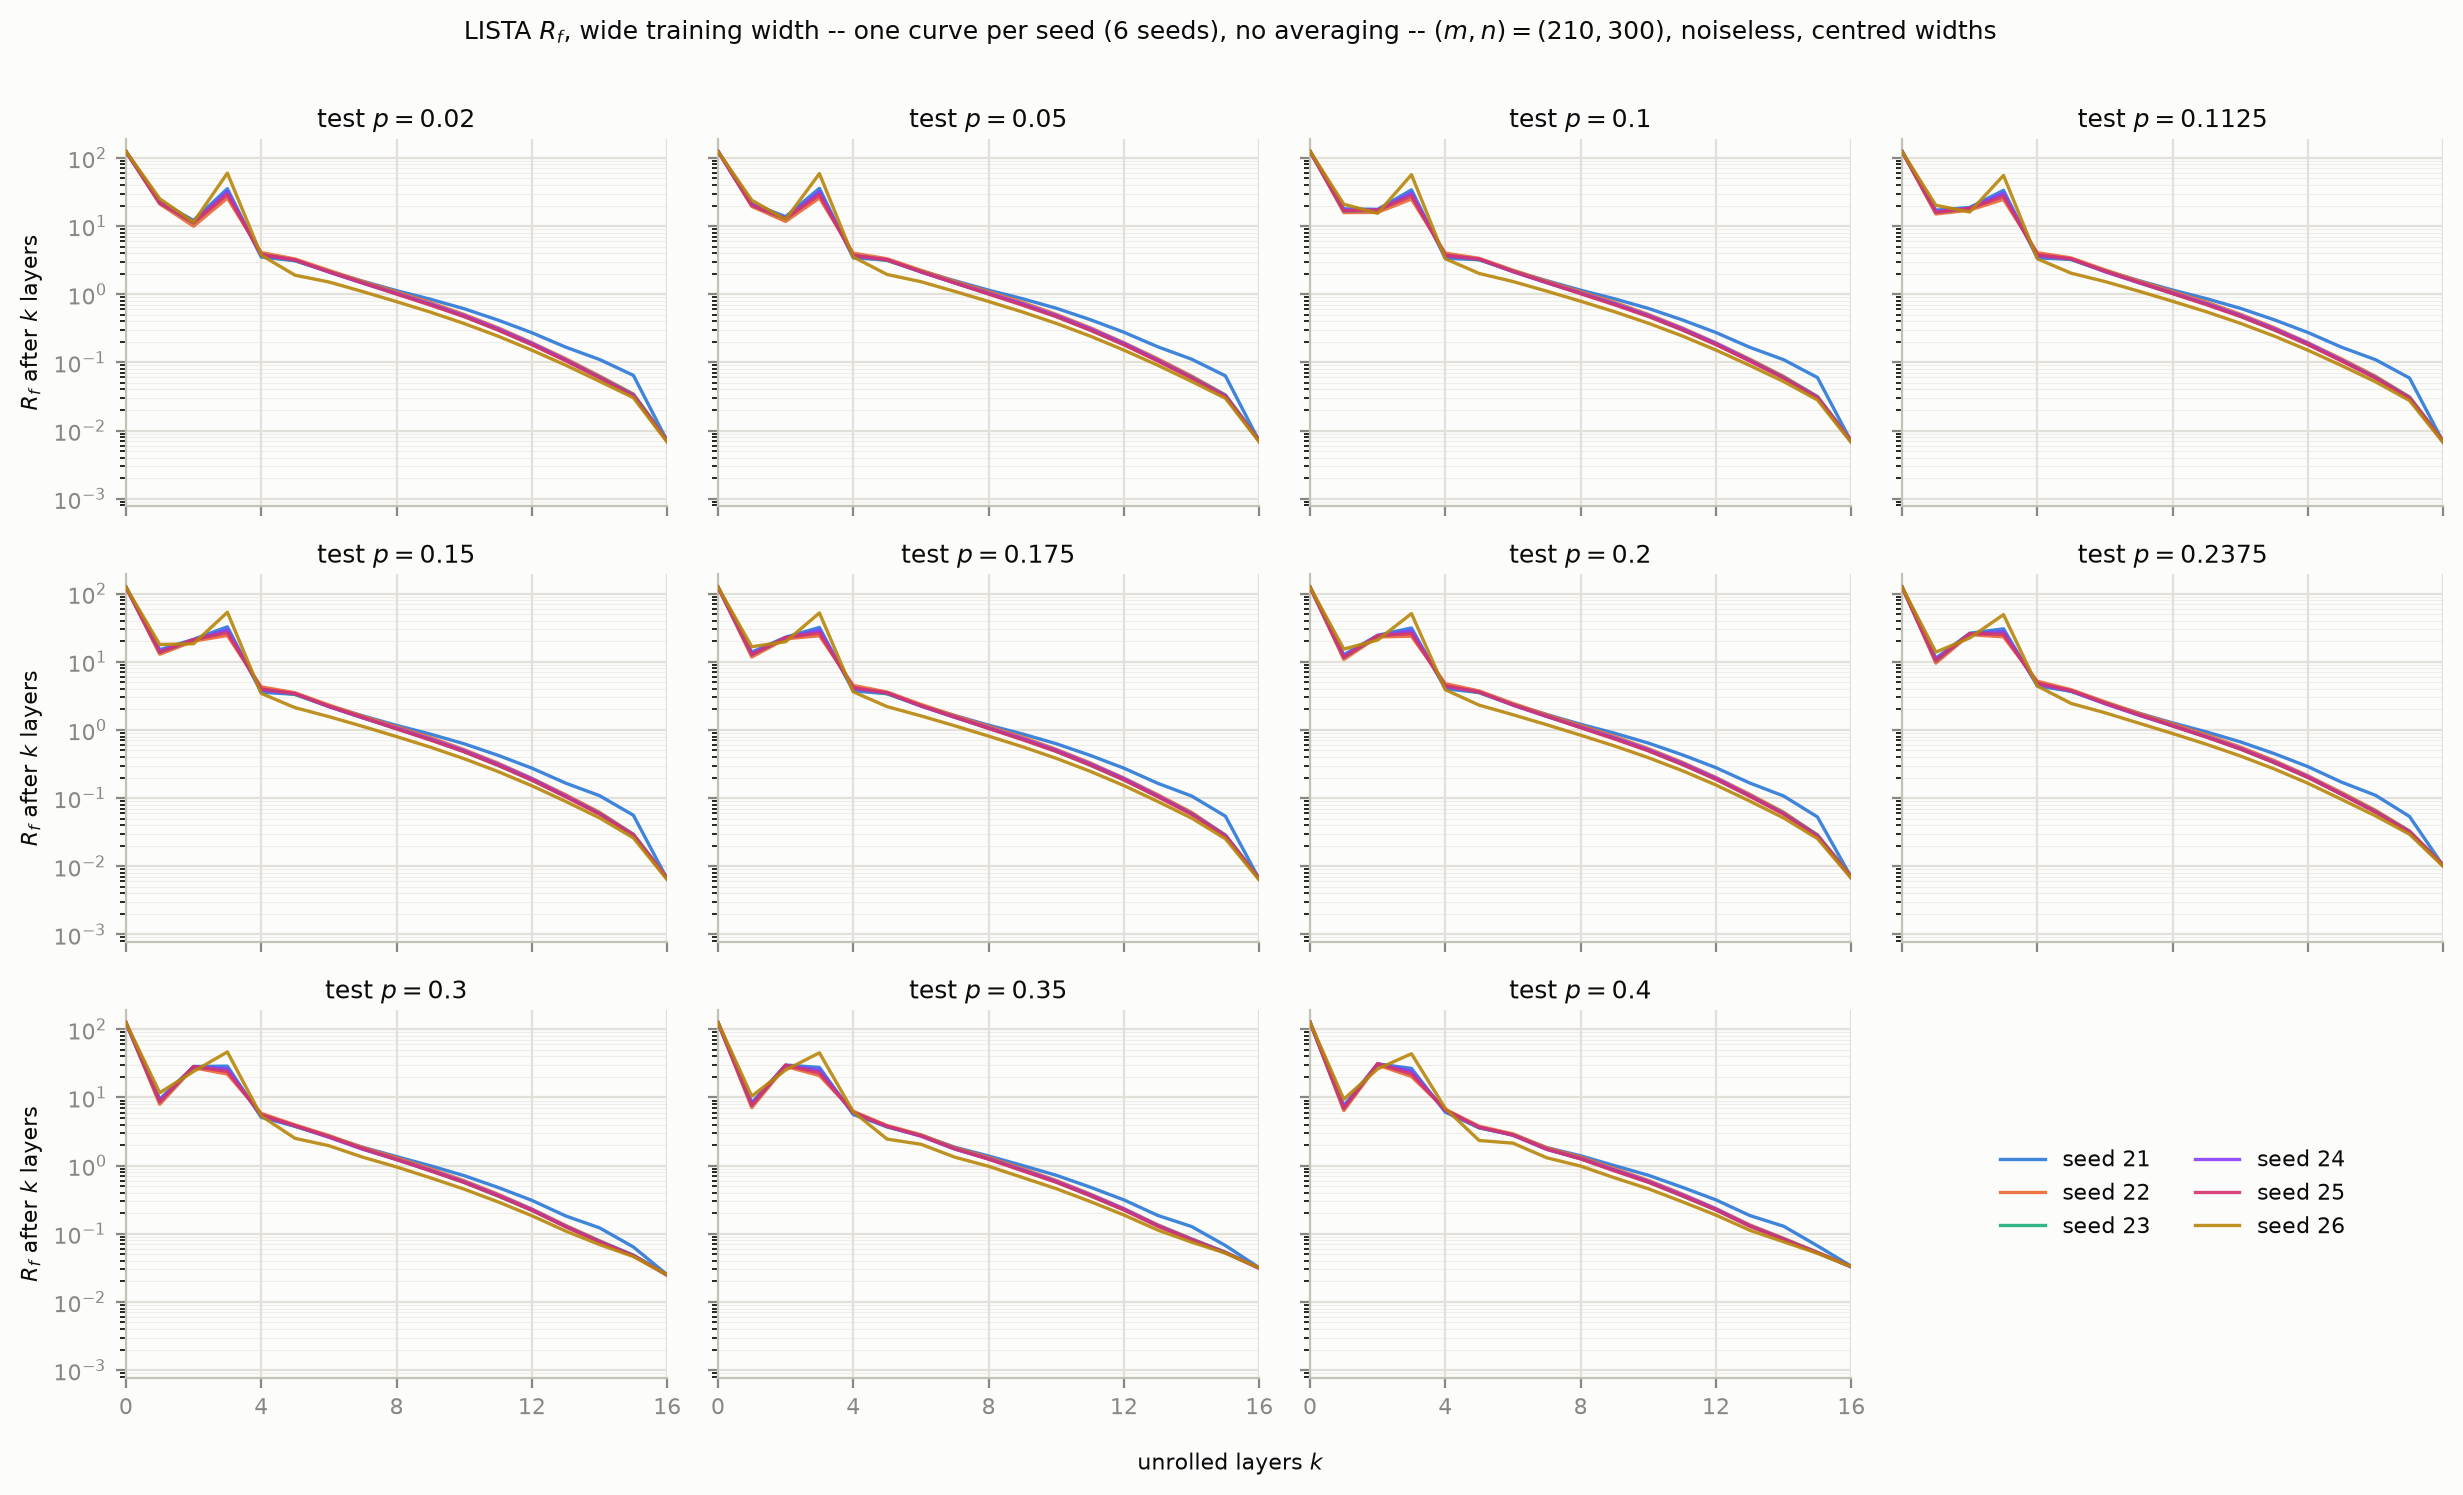
\includegraphics[width=\linewidth]{Figs/exp2_try3_210x300/lista_seed_curves_exp2_try3_210x300_wide.png}
  \caption{Wide ($p \in [0.05, 0.30]$)}
  \label{fig:lista-seed-curves-exp2-try3-210x300-wide}
\end{subfigure}\\[6pt]
\caption{LISTA, modified relative loss $R_f$ (Eq.~10) against unrolled layer $k$, $(m,n) = (210, 300)$, noiseless, centred widths. One curve per training seed (6 independently trained networks per width), no averaging; one panel per test sparsity $p$. $k = 0$ is the shared seeded start $x_0$, $k = 16$ the network's output. Unlike the model-free optimizer, every layer's weights are free, so the seeds may separate from the first layer on.}
\label{fig:lista-seed-curves-exp2-try3-210x300}
\end{figure}

\begin{figure}[htbp]
\centering
\begin{subfigure}[t]{\linewidth}
  \centering
  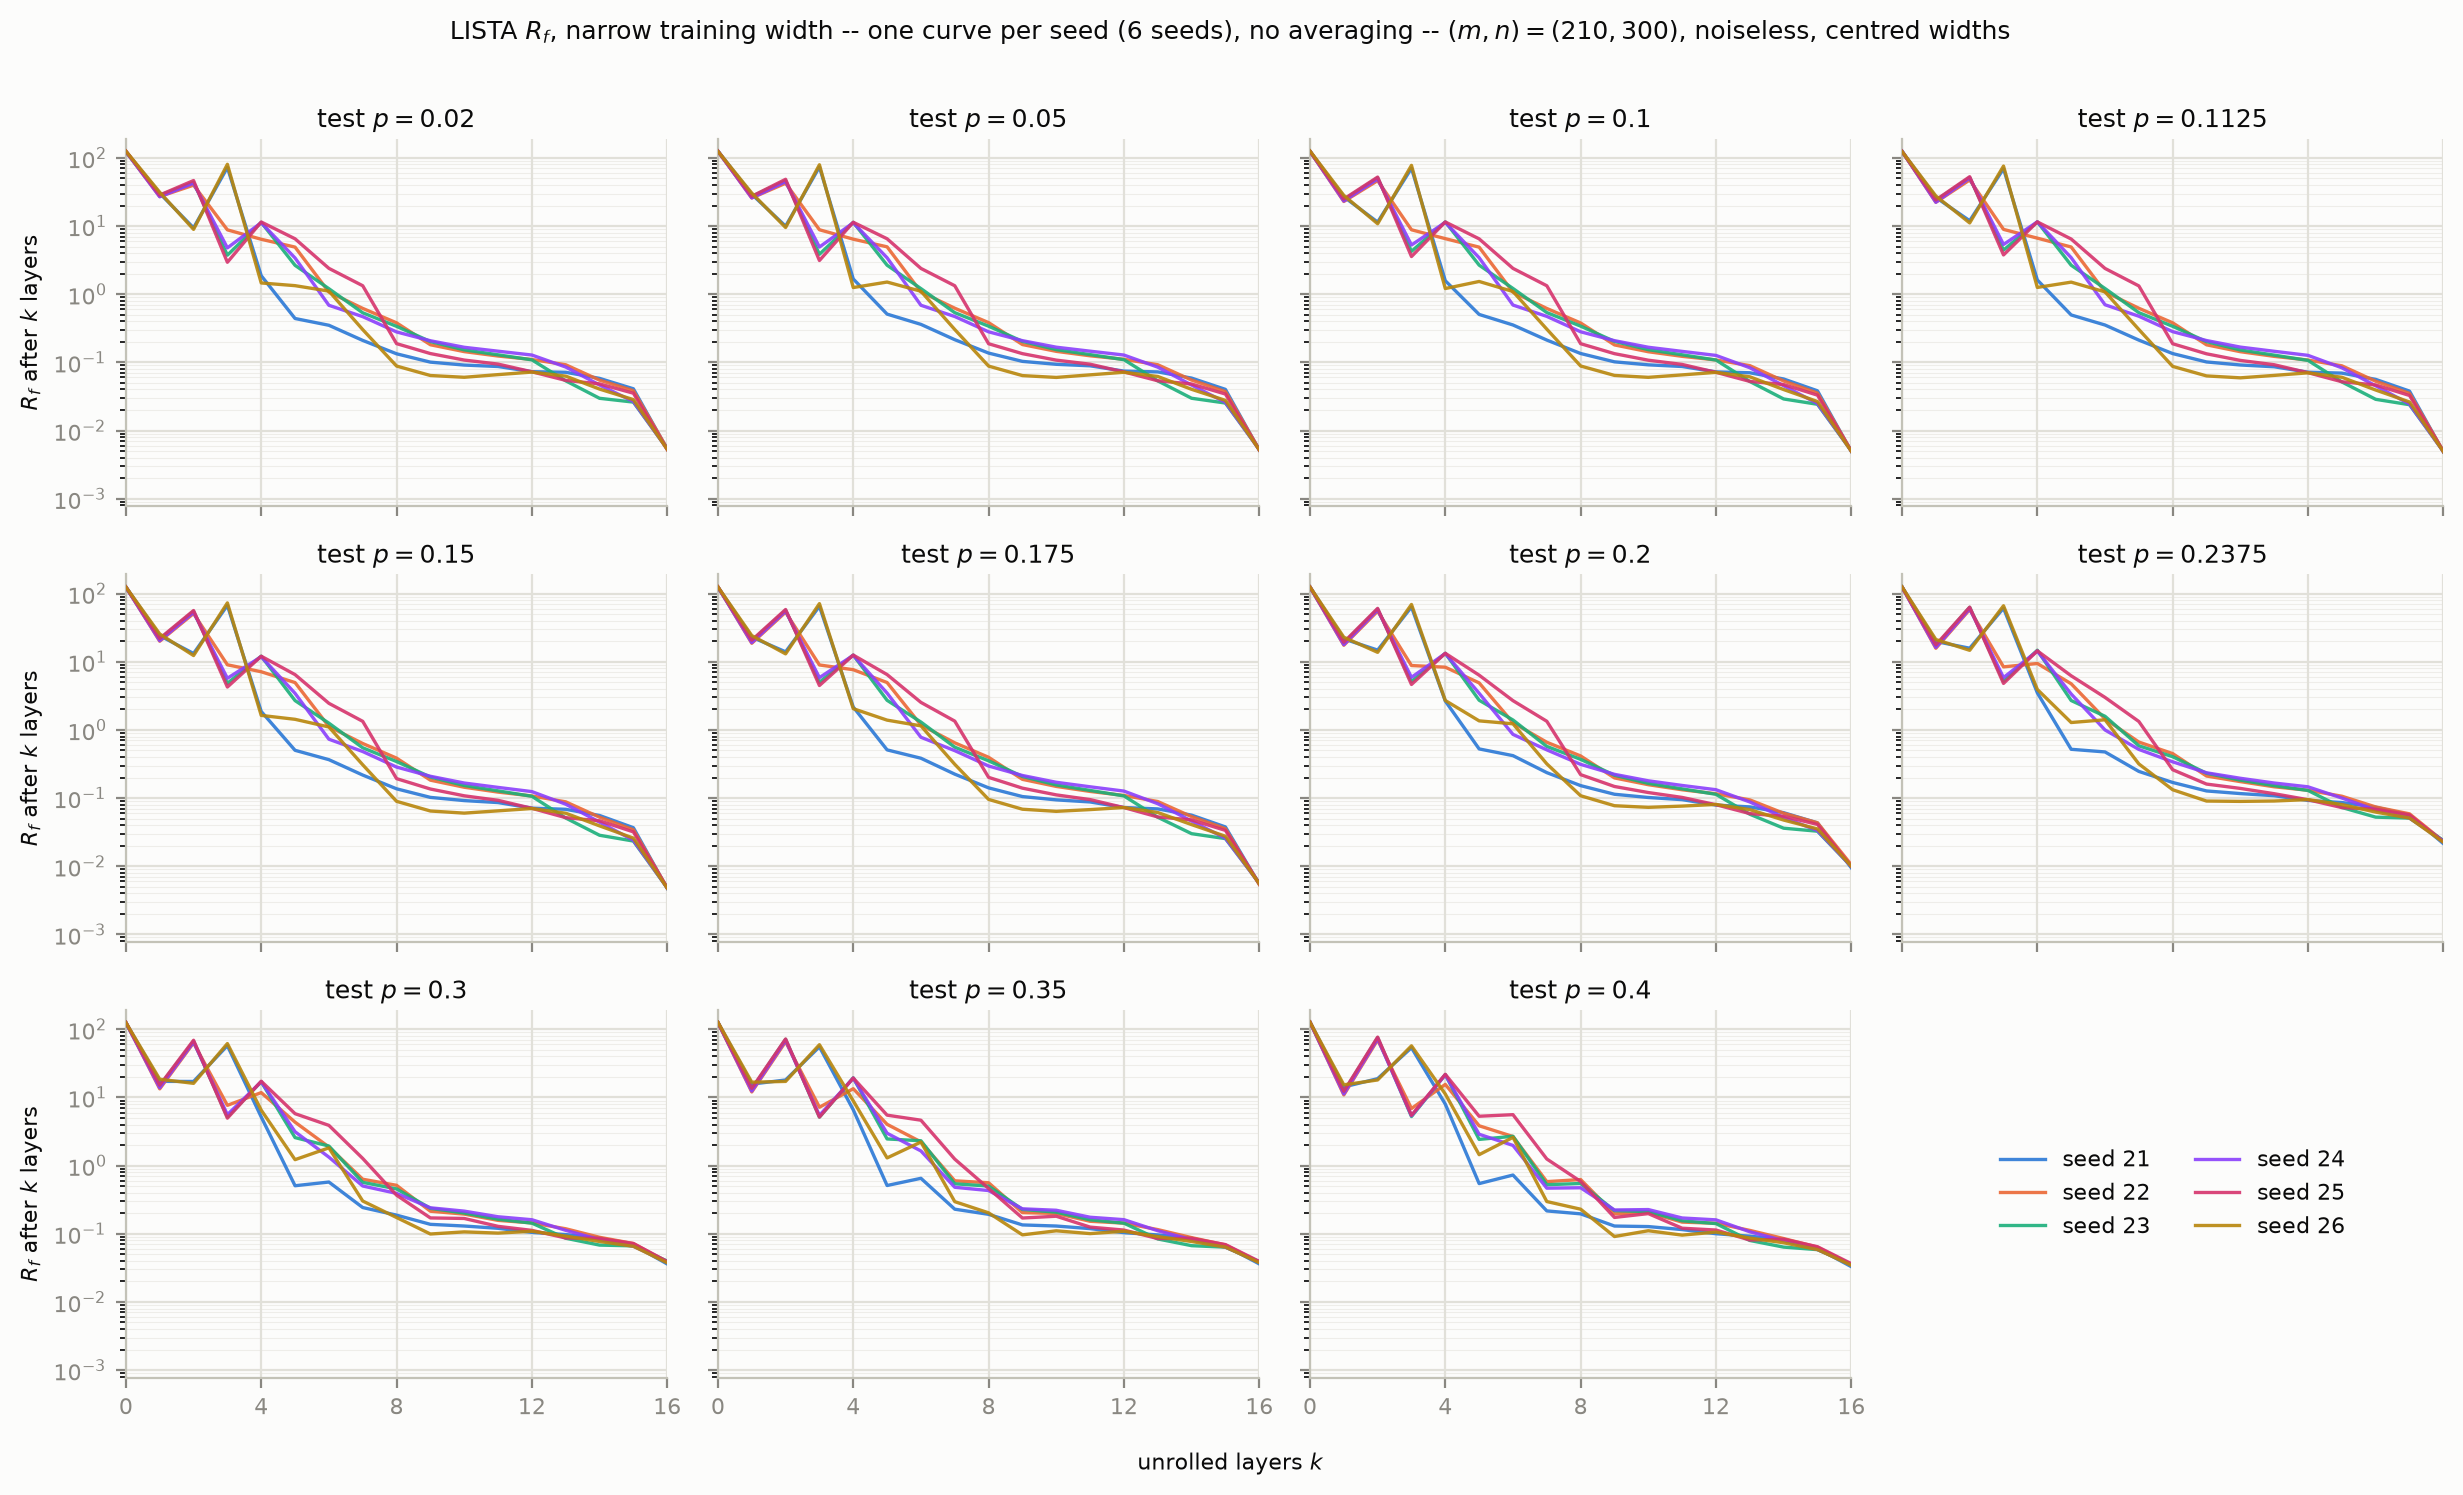
\includegraphics[width=\linewidth]{Figs/exp2_try3_210x300/lista_seed_curves_exp2_try3_210x300_narrow.png}
  \caption{Narrow ($p = 0.175$)}
  \label{fig:lista-seed-curves-exp2-try3-210x300-narrow}
\end{subfigure}\\[6pt]
\begin{subfigure}[t]{\linewidth}
  \centering
  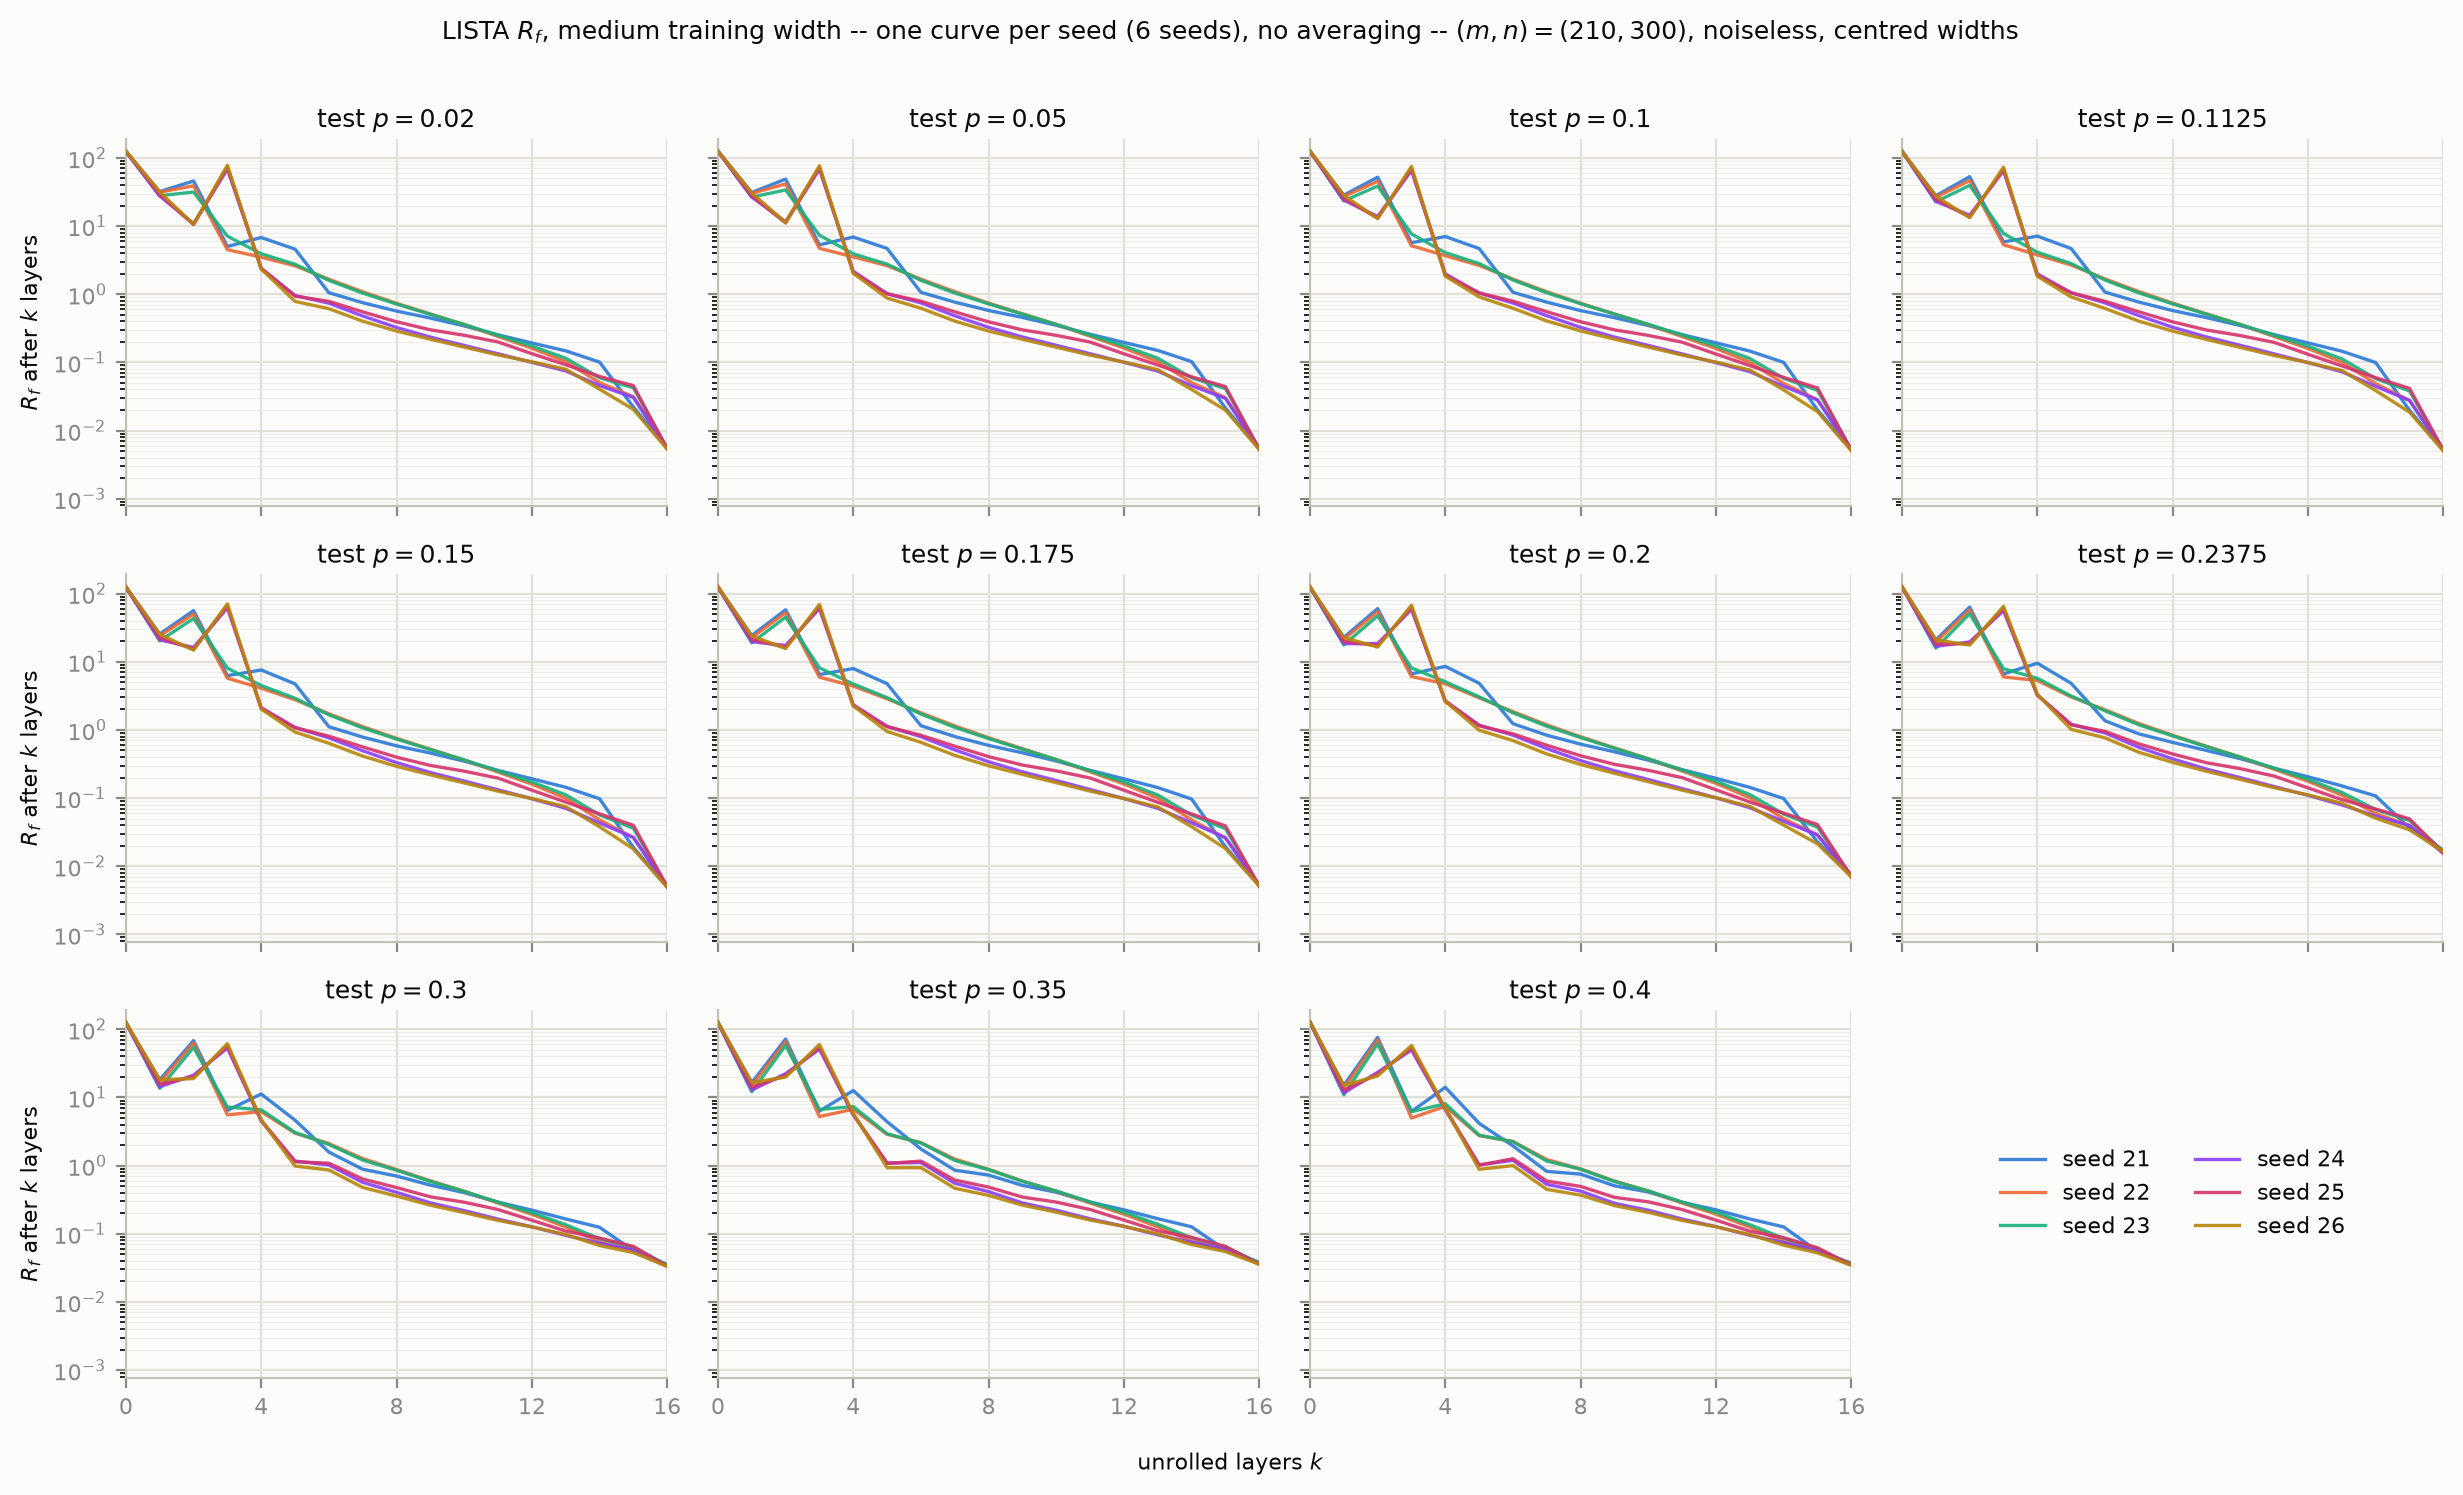
\includegraphics[width=\linewidth]{Figs/exp2_try3_210x300/lista_seed_curves_exp2_try3_210x300_medium.png}
  \caption{Medium ($p \in [0.1125, 0.2375]$)}
  \label{fig:lista-seed-curves-exp2-try3-210x300-medium}
\end{subfigure}\\[6pt]
\begin{subfigure}[t]{\linewidth}
  \centering
  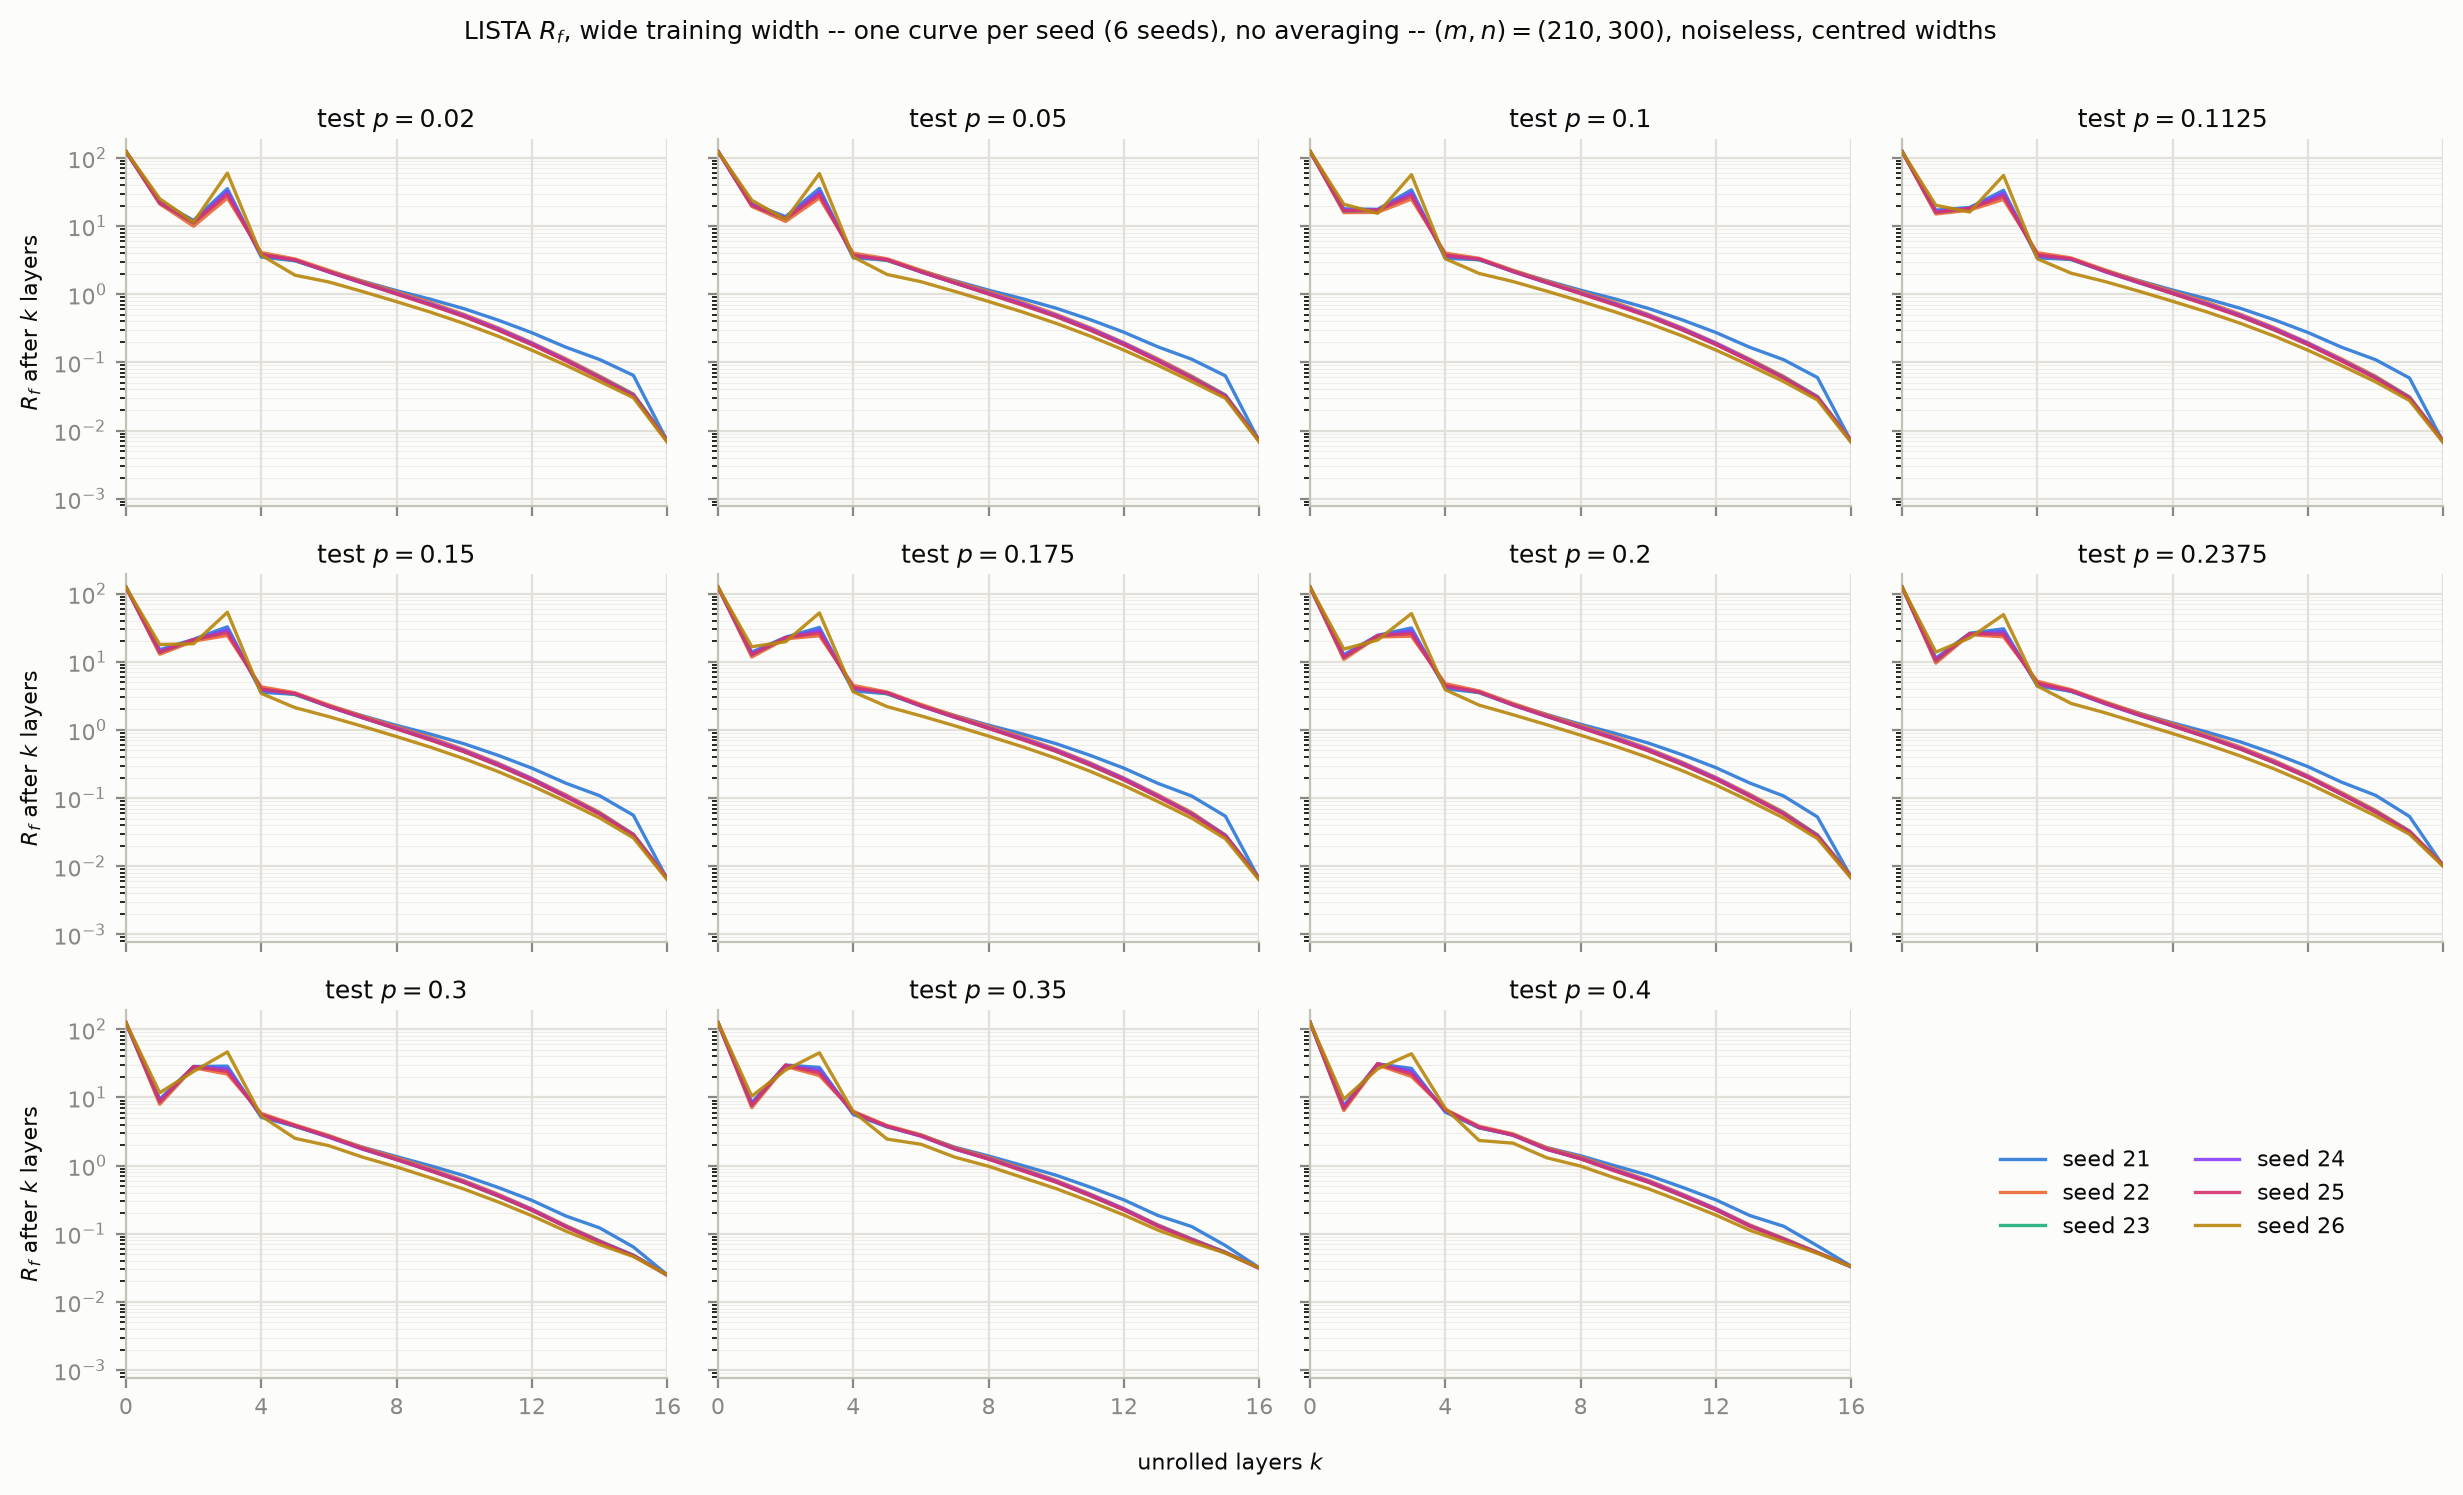
\includegraphics[width=\linewidth]{Figs/exp2_try3_210x300/lista_seed_curves_exp2_try3_210x300_wide.png}
  \caption{Wide ($p \in [0.05, 0.30]$)}
  \label{fig:lista-seed-curves-exp2-try3-210x300-wide}
\end{subfigure}\\[6pt]
\caption{LISTA, modified relative loss $R_f$ (Eq.~10) against unrolled layer $k$, $(m,n) = (210, 300)$, noiseless, centred widths. One curve per training seed (6 independently trained networks per width), no averaging; one panel per test sparsity $p$. $k = 0$ is the shared seeded start $x_0$, $k = 16$ the network's output. Unlike the model-free optimizer, every layer's weights are free, so the seeds may separate from the first layer on.}
\label{fig:lista-seed-curves-exp2-try3-210x300}
\end{figure}

\begin{figure}[htbp]
\centering
\begin{subfigure}[t]{\linewidth}
  \centering
  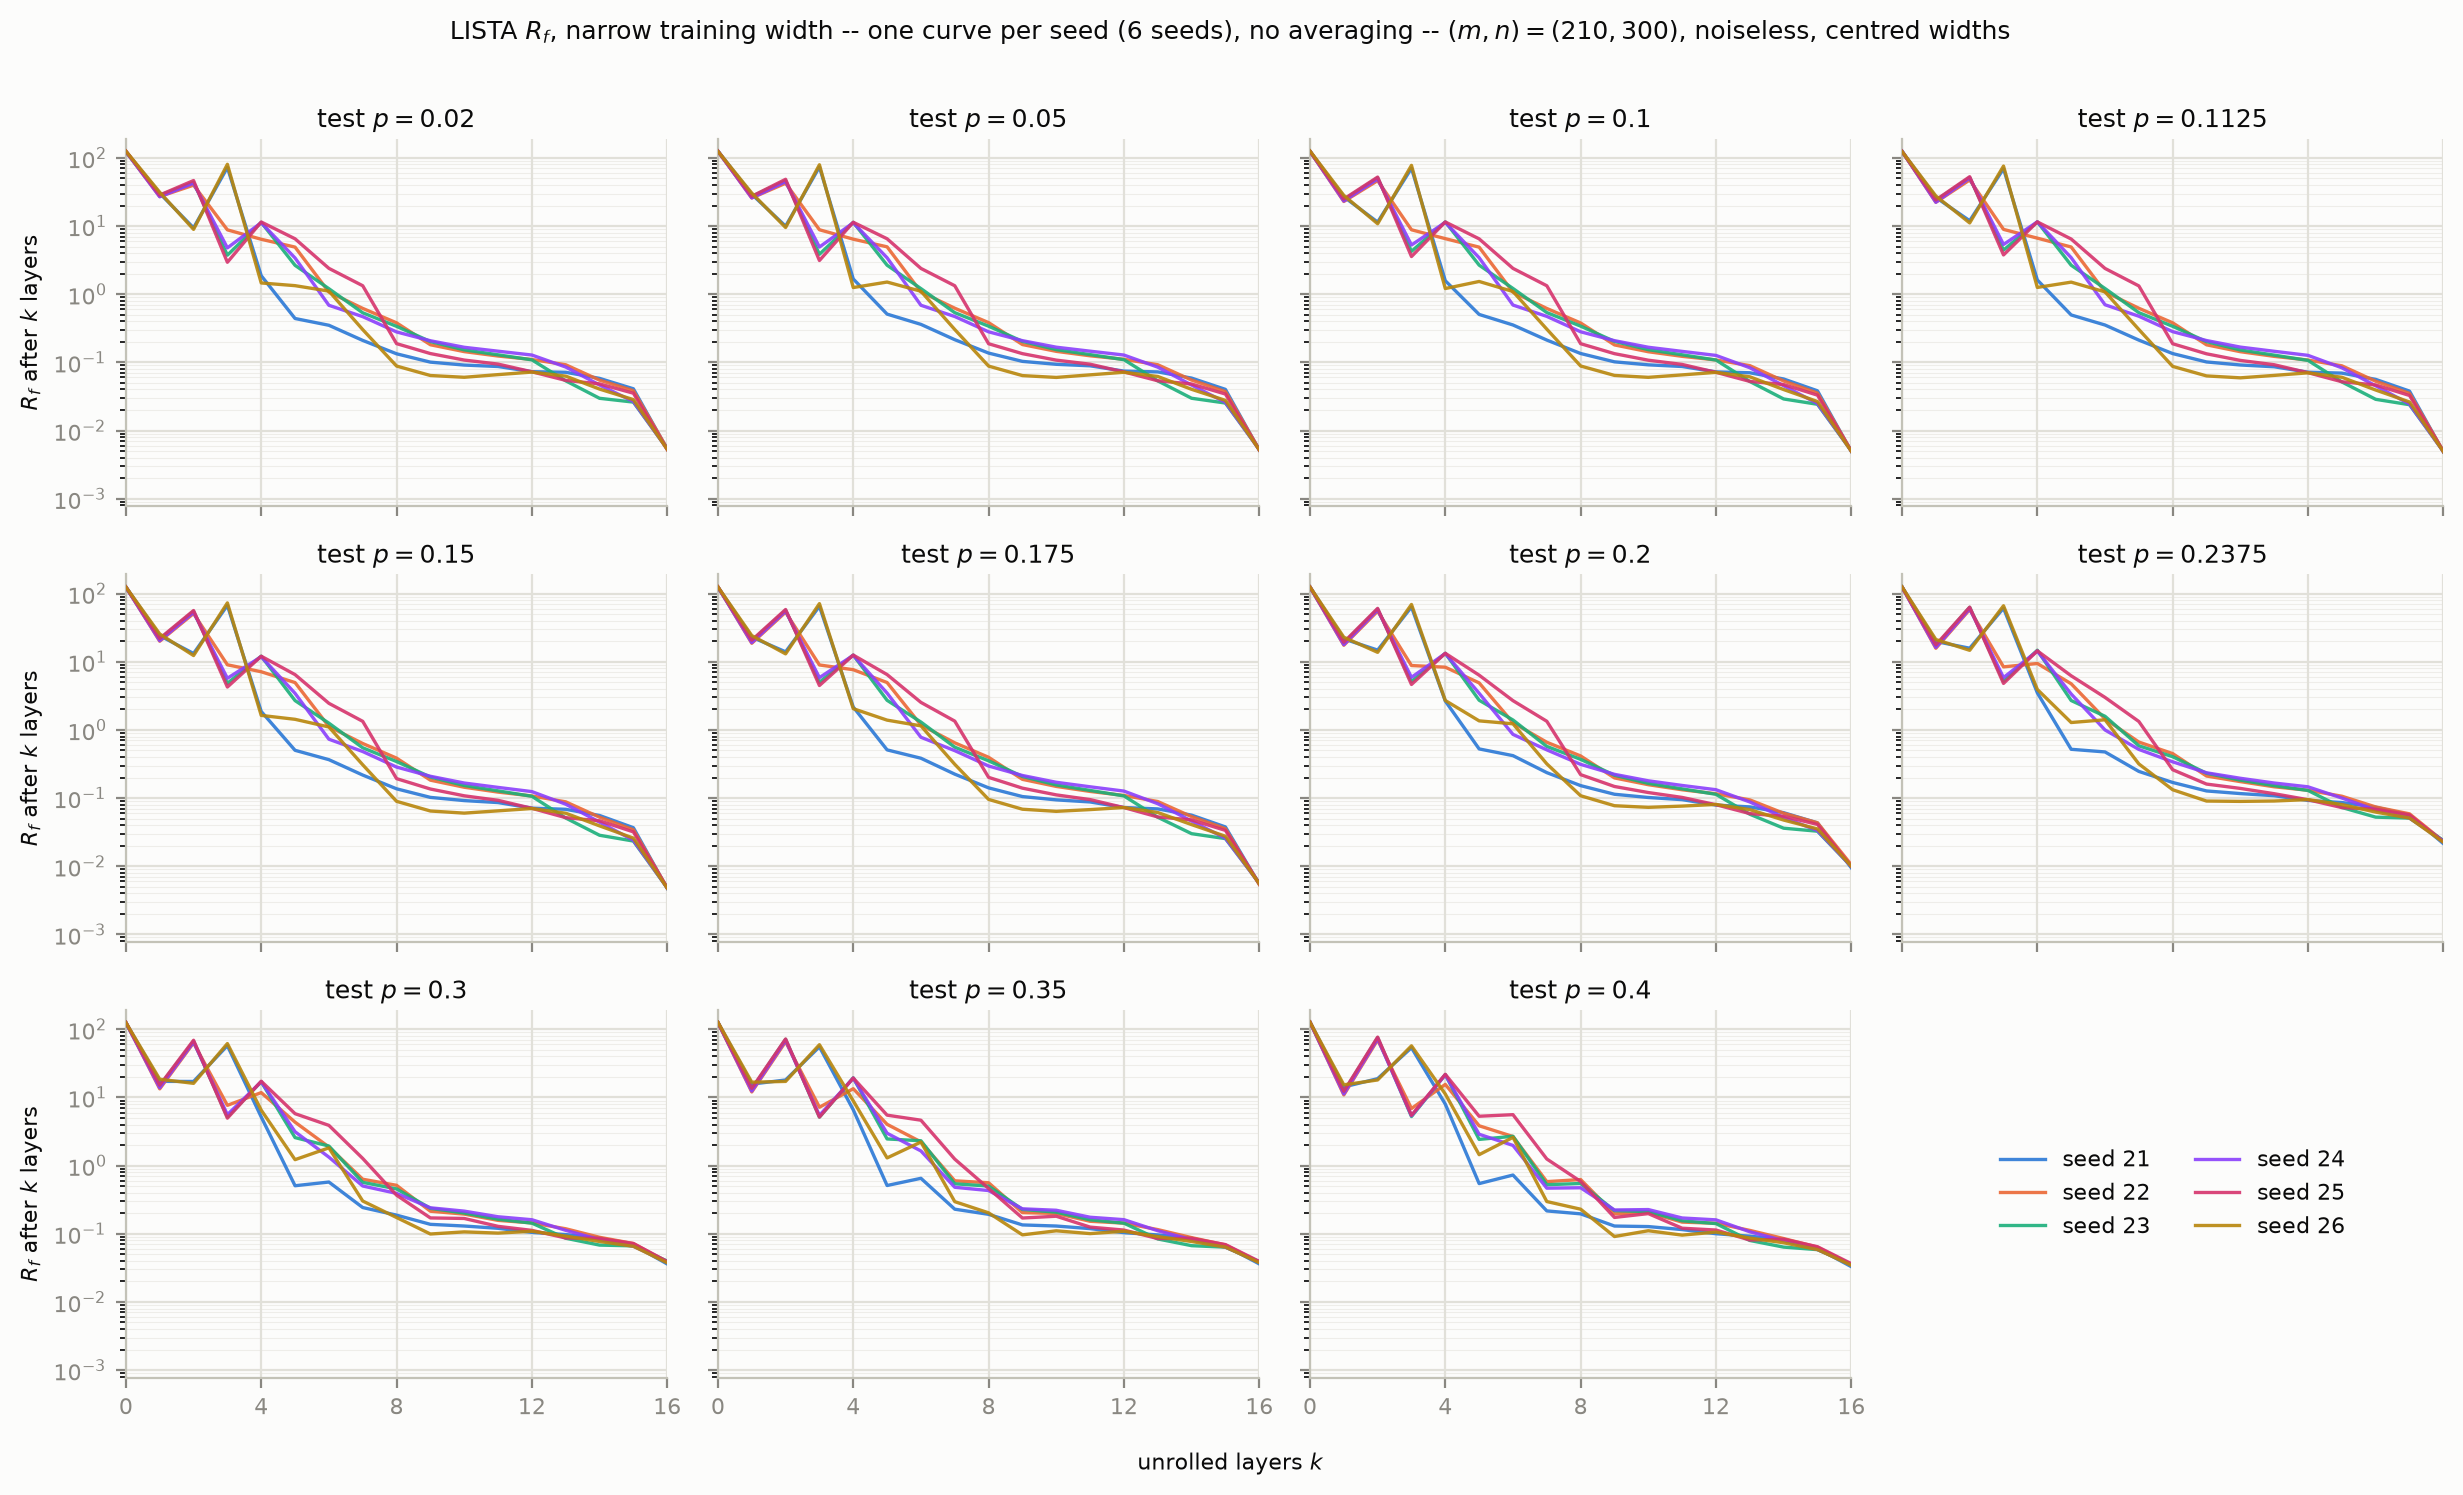
\includegraphics[width=\linewidth]{Figs/exp2_try3_210x300/lista_seed_curves_exp2_try3_210x300_narrow.png}
  \caption{Narrow ($p = 0.175$)}
  \label{fig:lista-seed-curves-exp2-try3-210x300-narrow}
\end{subfigure}\\[6pt]
\begin{subfigure}[t]{\linewidth}
  \centering
  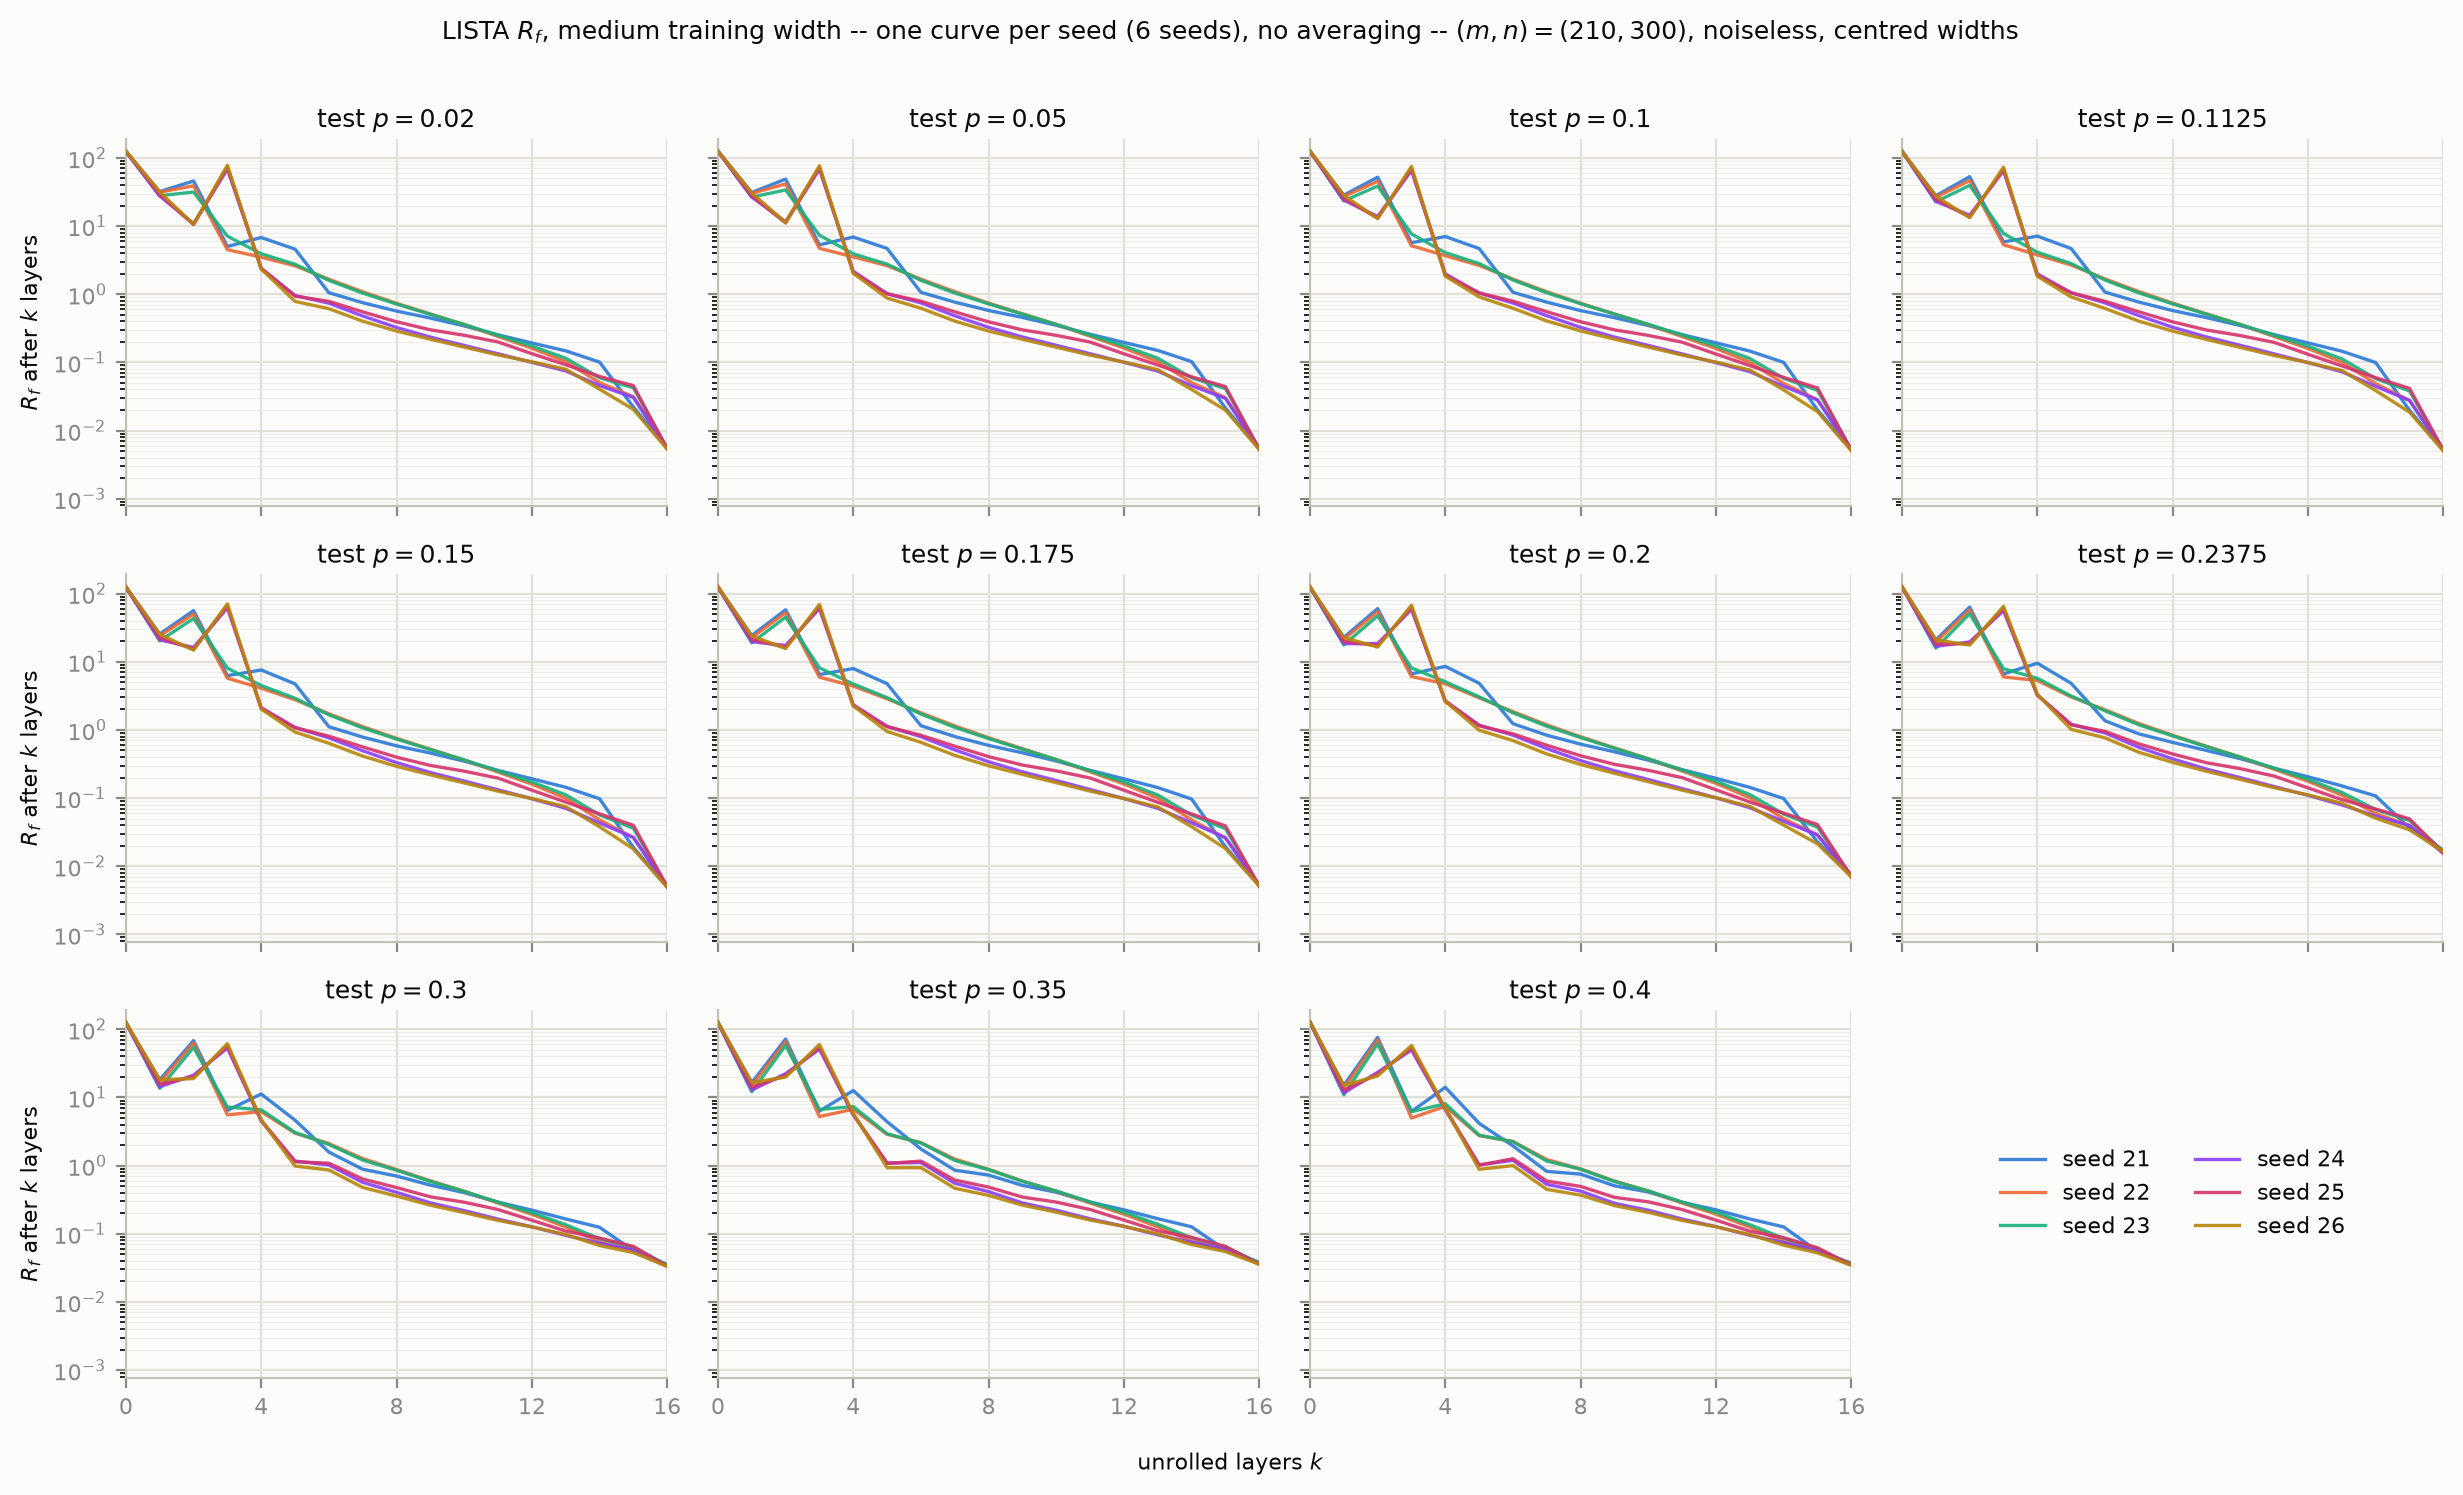
\includegraphics[width=\linewidth]{Figs/exp2_try3_210x300/lista_seed_curves_exp2_try3_210x300_medium.png}
  \caption{Medium ($p \in [0.1125, 0.2375]$)}
  \label{fig:lista-seed-curves-exp2-try3-210x300-medium}
\end{subfigure}\\[6pt]
\begin{subfigure}[t]{\linewidth}
  \centering
  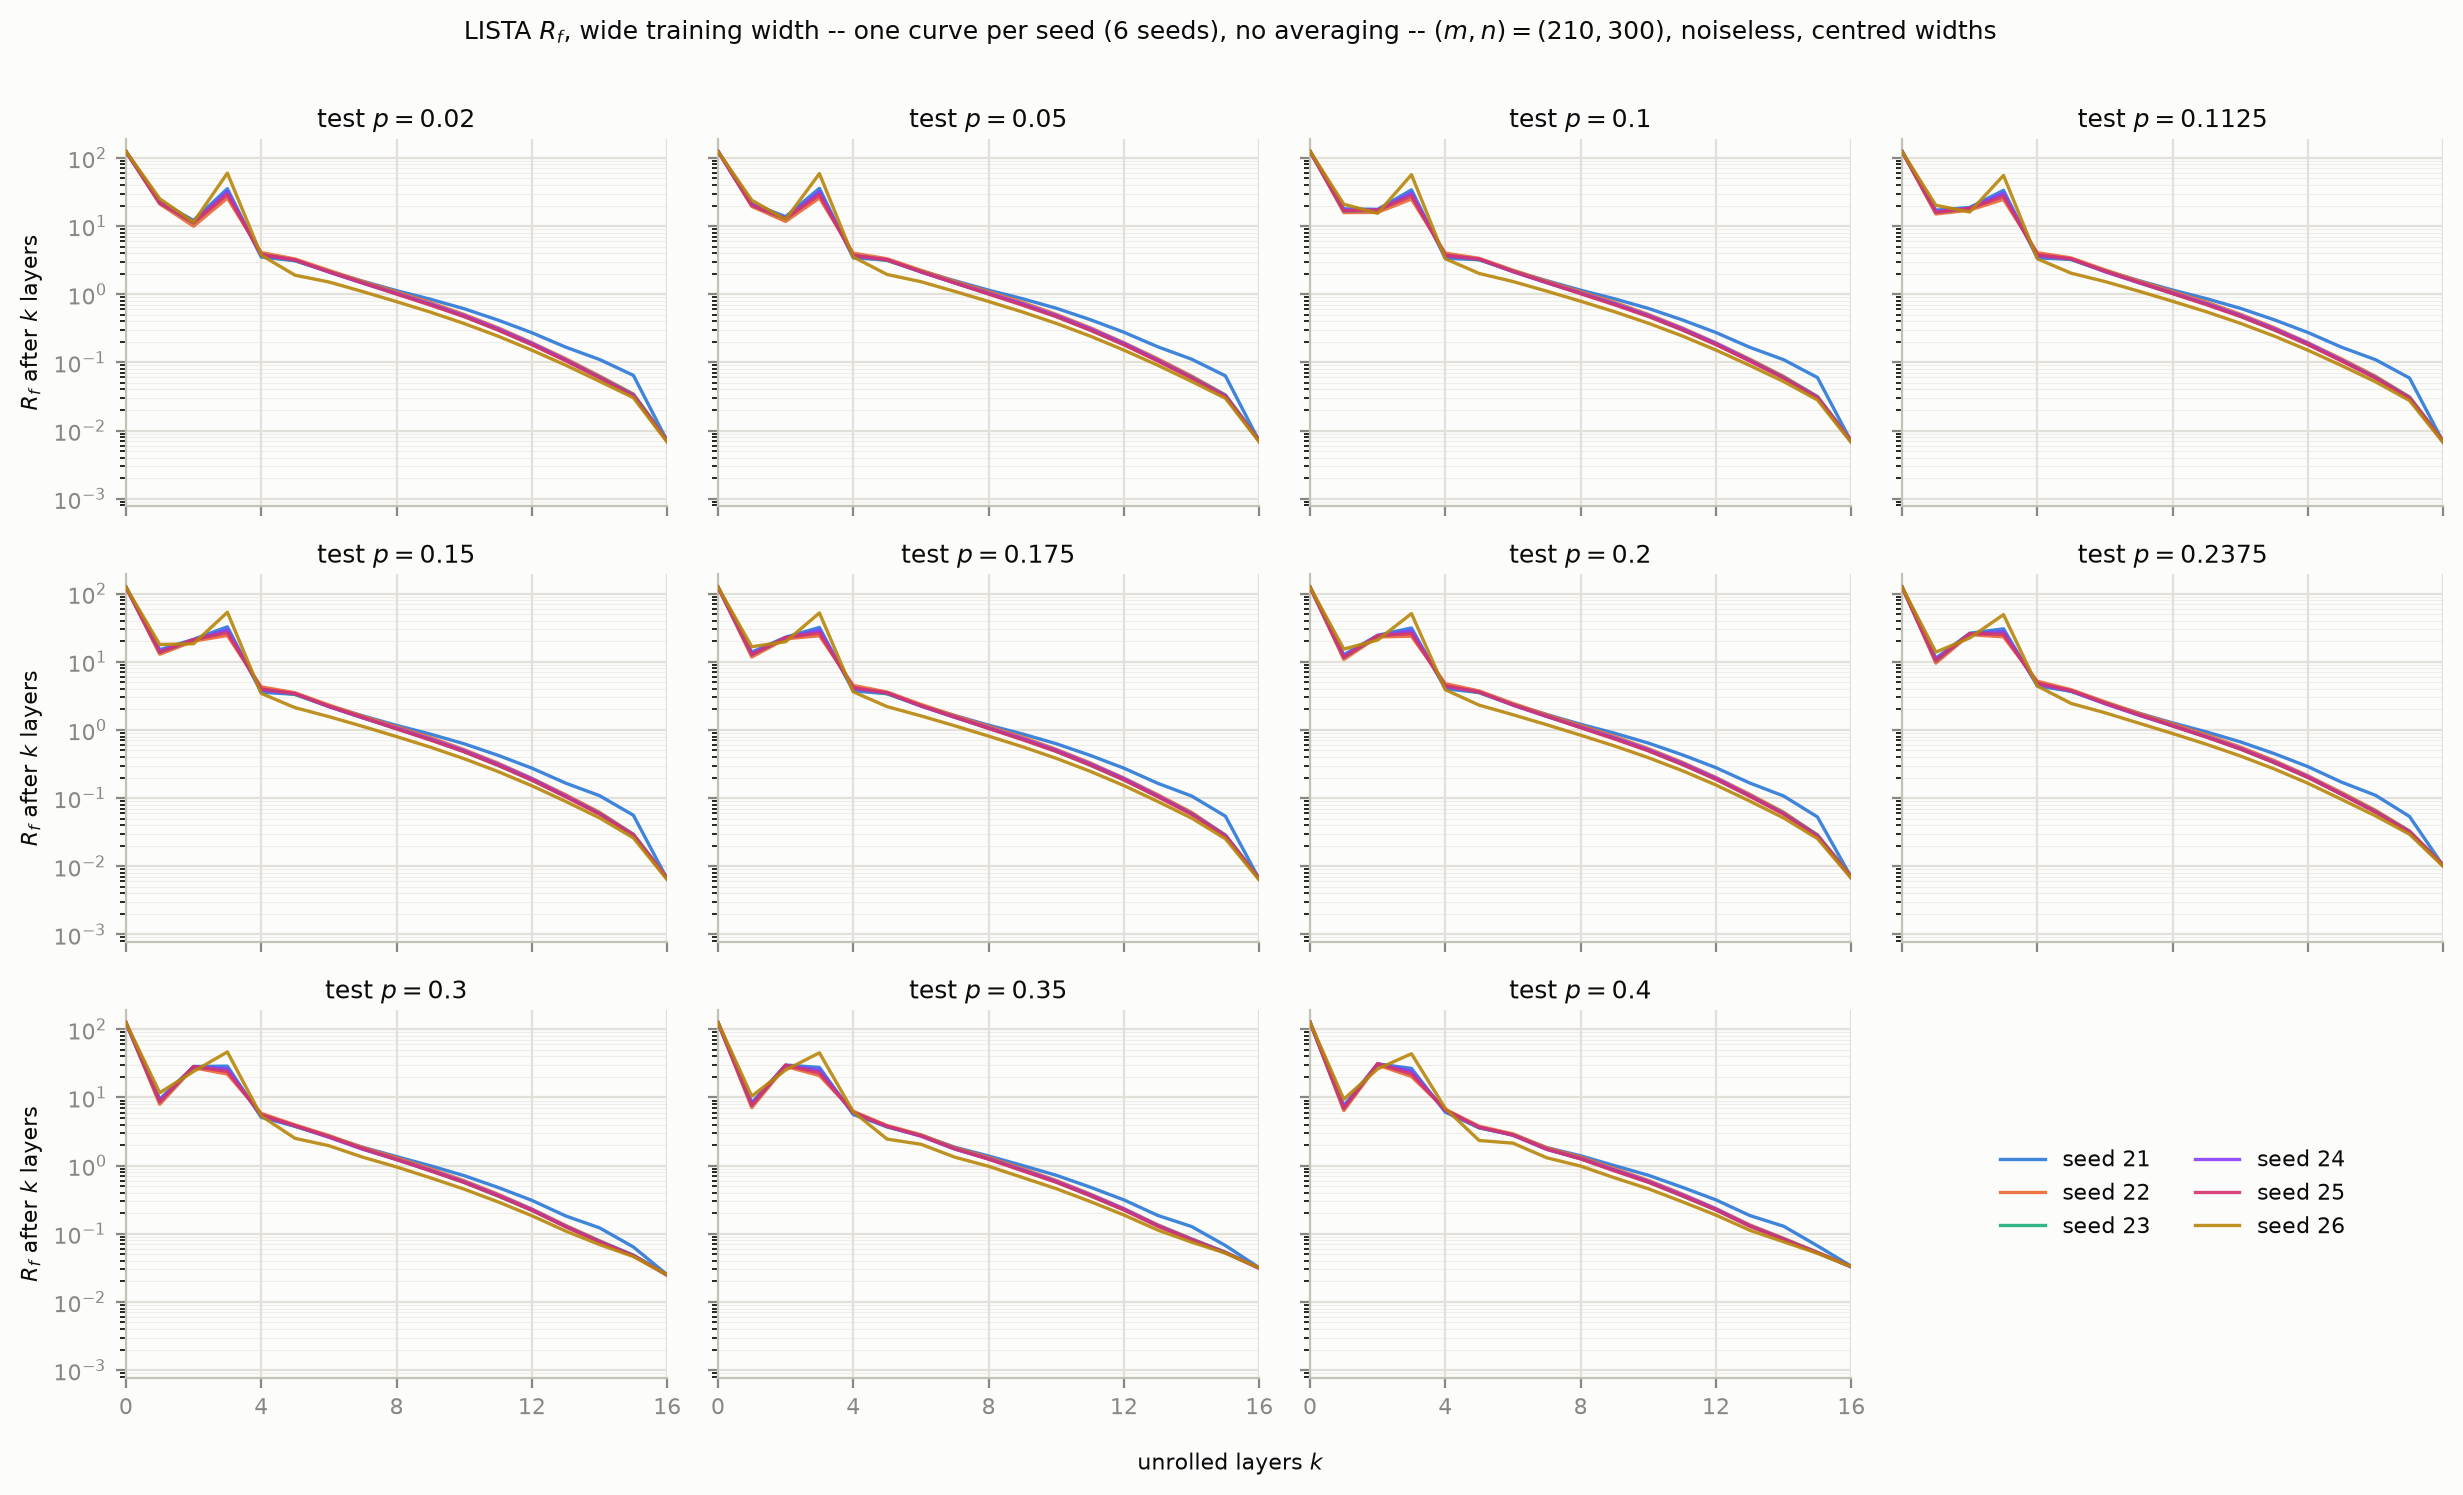
\includegraphics[width=\linewidth]{Figs/exp2_try3_210x300/lista_seed_curves_exp2_try3_210x300_wide.png}
  \caption{Wide ($p \in [0.05, 0.30]$)}
  \label{fig:lista-seed-curves-exp2-try3-210x300-wide}
\end{subfigure}\\[6pt]
\caption{LISTA, modified relative loss $R_f$ (Eq.~10) against unrolled layer $k$, $(m,n) = (210, 300)$, noiseless, centred widths. One curve per training seed (6 independently trained networks per width), no averaging; one panel per test sparsity $p$. $k = 0$ is the shared seeded start $x_0$, $k = 16$ the network's output. Unlike the model-free optimizer, every layer's weights are free, so the seeds may separate from the first layer on.}
\label{fig:lista-seed-curves-exp2-try3-210x300}
\end{figure}
